% !TEX encoding = UTF-8 Unicode
% !BIB TS-program = biber

\DocumentMetadata 
{
	lang		= en-US,
	pdfversion  = 1.7,
	pdfstandard = a-2b,
    pdfversion  = 2.0,
    pdfstandard = { ua-2, a-4f },
    tagging		= on,
}

%%%%%%%%%  Documentclass and options  %%%%%%%%%%%%%%%%%%%%%%%%%%%%%%%%%%%%%

\documentclass[fontset=termes-stix2,twosided]{mitthesis}

%%%%%%%%%  Packages used  %%%%%%%%%%%%%%%%%%%%%%%%%%%%%%%%%%%%%%%%%%%%%%%%%

%% Package for code listing
% \usepackage{listings}
\usepackage{verbatim}

%% Table related packages  
\usepackage{booktabs}% publication quality tables
\usepackage{array}% Additional options for column formats
\usepackage{dcolumn}% For alignment of numbers on the decimal place 
    \newcolumntype{d}[1]{D{.}{.}{#1}}
\usepackage{longtable}
	\setlength{\LTcapwidth}{\linewidth}

%% Package for improved typography
\usepackage[nopatch=footnote]{microtype}

%% Load this if using the two-column nomenclature format, \begin{nomenclature*}
\usepackage{multicol}

\usepackage{tabularx}


%%%%%%%%%  Graphics path (to figure files)  %%%%%%%%%%%%%%%%%%%%%%%%%%%%%%%%

\graphicspath{ {figures/} }% For details see: https://latexref.xyz/dev/latex2e.html#g_t_005cgraphicspath


%%%%%%%%%  Biblatex set-up  %%%%%%%%%%%%%%%%%%%%%%%%%%%%%%%%%%%%%%%%%%%%%%%%

%%   documentation is here: https://ctan.org/pkg/biblatex
%%   biblatex cheat sheet is here:   https://tug.ctan.org/info/biblatex-cheatsheet/biblatex-cheatsheet.pdf

%% Numerical citations of references
\usepackage[style=ext-numeric-comp,giveninits=true,maxbibnames=10,sorting=none,language=american]{biblatex}

% and make some changes to that style
	\renewcommand{\multicitedelim}{\addcomma}% removes space between consecutive cites to give [6,7], not [6, 7]
    \AtEveryBibitem{%
      \ifentrytype{article}{%
        \renewbibmacro{in:}{}% Removes "In:" for articles
		\renewcommand*{\jourvoldelim}{\addcomma\space}   % put comma after journal title
		\renewcommand*{\volnumdatedelim}{\addcomma\space}% put comma after volume info
		\renewbibmacro*{issue+date}{% Print date without parentheses around it
		\iffieldundef{issue}%
        	{}%
        	{\printfield{issue}%
         	\setunit*{\addcomma\space}
        	}%
			\printdate
		}
      }{}
    }
    %
	\renewbibmacro*{volume+number+eid}{%
        \printtext[bold]{\printfield{volume}}%    bold volume (issue number) , eid
%        \printtext[parens]{\printfield{number}}%  
        \iffieldundef{number}
          {} % do nothing
          {\printtext[parens]{\printfield{number}}} % print number in parentheses
        \setunit{\bibeidpunct}%
        \printfield{eid}
    }

\addbibresource{sources.bib}


%% to avoid split urls and stretched white space, you can make the bibliography ragged-right by uncommenting this:
%\AddToHook{cmd/bibsetup/after}{\raggedright}


%%%%%%%%%%  Option for "double spacing" %%%%%%%%%%%%%%%%%%%%%%%%%%%%%%%%%%%%

%% Back in the typewriter era, double spaced lines were convenient for editing with a pencil. 
%% In typography, the separation between lines is called "leading", and it is usually set in 
%% proportion to the font size (i.e., when the font is loaded).  If you really feel the need 
%% to change the line separation, the most attractive results will be obtained by changing the
%% leading in proportion to the the current font size, rather than just doubling the space.

%% The setspace package provides a tool for changing line separation. Use these two commands here:
%
\usepackage{setspace}%  documentation at https://ctan.org/pkg/setspace
\setstretch{1.1}% you can choose some other value for the stretch of space between lines
%
%% Use one or more of the these commands *AFTER* the frontmatter
%
% \onehalfspacing
% \doublespacing
% \singlespacing  % will turn these effects off (you can use these anywhere in the document)

%% The best result is usually to stay with the default leading (or to learn about latex font settings).


%%%%%%%%%%%  Metadata  %%%%%%%%%%%%%%%%%%%%%%%%%%%%%%%%%%%%%%%%%%%%%%%%%%%%%%%

% Most of the document metadata is created automatically. 
% The following items should be adjusted to match your work. <================= !!!!!!!!!!

\hypersetup{%
	pdfsubject={Using applied category theory to create a generalized framework for bus network redesigns that incorporates equitable factors},
	% Change this to briefly state topic of your thesis 
% 
	pdfkeywords={Massachusetts Institute of Technology, MIT, Diego Temkin, public transit planning, transportation network design, accessibility, applied category theory, mixed-integer linear programming},
	% Add keywords that will help search engines and libraries to find your work.
	% Includes the name[s] of the author[s] 
	% (If you used \DocumentMetadata at line 14, you can just put "\CopyrightAuthor," for the names.)
%
	% pdfurl={},
	% If you have a url for the thesis, put it here. Otherwise delete this.
	% (MIT Libraries will put your thesis in DSPACE with a persistent url after you submit it.)
%	
	pdfcontactemail={dtemkin@alum.mit.edu},
	% You can put a [permanent] email address into the metadata, if you like.
	% Otherwise delete this.
%
	% pdfauthortitle={},
	% If you have a title (e.g., Prof. Dr.-Ing.), you can include it here.
}

%%%%%%%%%%%%  Math operators %%%%%%%%%%%%%%%%%%%%%%%%%%%%%%%%%%%%%%%%%%%%%%%%%%%%

% These commands declare two math operators, \erf{..} and \erfc{..} using mathtools
% note: * form produces automatic delimiter scaling; optional argument sets size manually, e.g. [\bigg]
% See Table 1.1 in Chapter 1

\DeclareMathOperator{\Erf}{erf}
\DeclareMathOperator{\Erfc}{erfc}
\DeclarePairedDelimiterXPP\erf[1]{\Erf\mkern1mu}(){}{#1}% increase to 2mu with stix2 font
\DeclarePairedDelimiterXPP\erfc[1]{\Erfc\mkern1mu}(){}{#1}

%%%%%%%%%%%% Content that you need to write follows! %%%%%%%%%%%%%%%%%%%%%%%%%%%%

\includeonly{acknowledgments,intro,litreview,methods,results,discussion,conclusions,stakeholder,math,mcdpl}
%   for usage of includeonly, see https://latexref.xyz/_005cinclude-_0026-_005cincludeonly.html

% ACRONYMS

% for list of acronyms
\usepackage[nomain, acronym, toc, section=chapter, numberedsection=autolabel, nohypertypes={acronym}]{glossaries}

\makeglossaries

\newacronym{acs}{ACS}{American Community Survey}
\newacronym{afc}{AFC}{Automatic Fare Collection}
\newacronym{afi}{AFI}{Accessibility Fairness Index}
\newacronym{av}{AV}{autonomous vehicle}
\newacronym{avl}{AVL}{Automatic Vehicle Location}
\newacronym{bird}{BiRD}{Biobjective Routing Decomposition}
\newacronym{bps}{BPS}{Boston Public Schools}
\newacronym{bra}{BRA}{Bus Routing Algorithm}
\newacronym{cdpi}{CDPI}{Co-Design Problems with Implementation}
\newacronym{cvrp}{CVRP}{Capacitated Vehicle Routing Problem}
\newacronym{ej}{EJ}{Environmental Justice}
\newacronym{fps}{FPS}{Framingham Public Schools}
\newacronym{fta}{FTA}{Federal Transit Administration}
\newacronym{gps}{GPS}{Global Positioning System}
\newacronym{gqap}{GQAP}{Generalized Quadratic Assignment Problem}
\newacronym{gtfs}{GTFS}{General Transit Feed Specification}
\newacronym{ilp}{ILP}{integer linear programming}
\newacronym{lbh}{LBH}{largest-bus heuristic}
\newacronym{lp}{LP}{linear program}
\newacronym{mbta}{MBTA}{Massachusetts Bay Transportation Authority}
\newacronym{mcdp}{MCDP}{Monotone Co-Design Problem}
\newacronym{mdpi}{MDPI}{Monotone Design Problem with Implementation}
\newacronym{milp}{MILP}{Mixed-Integer Linear Program}
\newacronym{mwrta}{MWRTA}{MetroWest Regional Transit Authority}
\newacronym{od}{OD}{origin-destination}
\newacronym{osm}{OSM}{OpenStreetMap}
\newacronym{sbrp}{SBRP}{School Bus Routing Problem}
\newacronym{stsp}{STSP}{School Time Selection Problem}


\renewcommand{\chapterautorefname}{Chapter}
\renewcommand{\sectionautorefname}{Section}

%%%%%%%%%%%%%%  End preamble %%%%%%%%%%%%%%%%%%%%%%%%%%%%%%%%%%%%%%%%%%%%%%%%%%%%%%%%%%%%%%%%%%%%%
%%%%%%%%%%%%%%%%%%%%%%%%%%%%%%%%%%%%%%%%%%%%%%%%%%%%%%%%%%%%%%%%%%%%%%%%%%%%%%%%%%%%%%%%%%%%%%%%%%

\begin{document}

\title{Reimagining Urban Bus Operations: Using Category Theory to Create a Generalizable Framework for Bus Network Redesigns Incorporating Equitable Factors}

\Author{Diego Temkin}{Department of Urban Studies and Planning}
\Degree{Bachelor of Science in Planning}{Department of Urban Studies and Planning}

\Supervisor{Jim Aloisi}{Lecturer of Transportation Policy and Planning}[Department of Urban Studies and Planning]
\Acceptor{Justin Steil}{Associate Professor of Law and Urban Planning}{Department of Urban Studies and Planning, UG Committee Chair} % \\ \> Third title}

\DegreeDate{May}{2026}
\ThesisDate{May 15, 2026}

% \Reader{Riccardo Fiorista}{PhD student in Transportation, Department of Civil and Environmental Engineering (CEE) and Laboratory for Information andDecision Systems (LIDS)}

\CClicense{CC BY-NC-ND 4.0}{https://creativecommons.org/licenses/by-nc-nd/4.0/}


%%%%%%%  Solutions for overflowing titlepage  %%%%%%%%%%%%%%%%%%%%%%%%%%%%%%%%%%%%%%%%%%%%%%%%%%%

% If your title page is overflowing (from too many names, degrees, etc.):
%
% (a) you can reduce the 12pt and 18pt skips between various blocks to 6pt with this command:
%
% \Tighten
%
% (b)  you can scale down the Signature block at the bottom with this command:
%
% \SignatureBlockSize{\small}  %or this one \SignatureBlockSize{\footnotesize}
%
% (c) you can put the acceptor name and title onto two lines, rather than three like this:
%
% \Acceptor{Tertius Castor}{Professor and Graduate Officer, Department of Research}{}
%
% (d) you can change the font size of the author name[s] with
%
%	\AuthorNameSize{\normalsize}
%
% (e) and you can omit any previous degrees from the title page, instead mentioning them in the biographical sketch

% Also, if you prefer to keep the text toward the top of the page with most white space at the bottom, you
% can use this command to squash all of the vertical glue (stretchy space) with this command:
%
% \Squash 
%
% This command is useful when the text has not already reach the bottom of the page, since the glue gets squashed automatically
% when the page is too full.


%%%%%%%%%%%%%%%%%%%%%%%%%%%%%%%%%%%%%%%%%%%%%%%%%%%%%%%%%%%%%%%%%%%%%%%%%%%%%%%%%%%%%%%%%%%%%%%%%

%%% Make titlepage
\maketitle

%%%%%%%%% Content that you need to write follows! %%%%%%%%%%%%%%%%%%%%%%%%%%%%%%%%%%%%%%%%%%%%%%

% \includeonly{acknowledgments,biography,chapter1,chapter2,...,appendixa,...} 
%   for usage of includeonly, see https://latexref.xyz/_005cinclude-_0026-_005cincludeonly.html


%%% Frontmatter (write this material in the mentioned files)  %%%%%%%%%%%%%%%%%%%%%%%%%%%%%%%%%%%

% The abstract environment creates all the required headings and footers. 
% You only need to the text of the abstract in the file abstract.tex
\begin{abstract}
	% Approximately 500 words or less; try not to use formulas or special characters
% If you don't want an initial indentation, do \noindent at the start of the abstract

Despite advances in mobility technology, cities still struggle to design bus systems that are efficient, equitable, and adaptable to evolving urban needs. Computational bus service design aims to identify bus routes which match historic ridership demand while complying with requirements from the built environment, expected reliability, equity, efficiency, and environmental impact, but very little work has been done on integrating equity analyses into these computational network optimizations.  In this thesis, I explore how to conduct bus network redesigns in a method that balances service quality and cost with equity and accessibility factors. This is done by creating a blueprint using an applied category theory framework that can take into account transit network data and capture the complex interplay of various stakeholders. This formalism will assist city planners, transit operators, and passengers, and is applied as a case study to a real-world transit agency in Framingham, MA to assess feasibility and accuracy, as well as to identify areas for further improvement and research. % use \input rather than \include because we're inside an environment
\end{abstract}

%% acknowledgments.tex

% From mitthesis package
% Version: 1.02, 2024/06/19
% Documentation: https://ctan.org/pkg/mitthesis

\chapter*{Acknowledgments}
\pdfbookmark[0]{Acknowledgments}{acknowledgments}

\begin{itemize}
    \item Family (Mami, Papi, Hali, Aby, Guelis, Papa) for always believing in me and pushing me to succeed
    \item Friends and upperclassmen at MIT for letting me rant at 2am and giving me space to be myself (Simmons ppl, gay agenda, 1E, Stickman, DormCon, SIPB, WMBR, TDC, Lillian)
    \item Riccardo and Gioele for introducing me to new fields and being patient as I blundered my way through them
    \item Jim for advising and giving me feedback when I needed it most
    \item Cong Cong and John Akula for helping me through my first ever research experiences
    \item Staff at MIT for always supporting me when I didn't know who to turn to (Connor, Amanda, Kat H, Kat W, Helen, Tasha, Elise, Ashley, Maddie Garcia, Mich, Rishi, Briana)
    \item Those at Volpe and WMATA who always made me feel welcome even when it felt like the world was crashing down (Volpe 331/336: Mark, Carmen, Mac, April, Mikayla, Michael, Scott, Ian, Rachael) (WMATA: Doojin, Billy, Jim)
    \item Teachers before MIT who thought I could make it (Ms. Bay, Ms. Camarena, Mr. D, everyone at SciTech)
\end{itemize}












% acknowledgments.tex (.tex extension is presumed by \include) 

%%% Table of contents and lists of stuff (delete unused lists, i.e., if no tables or figures) %%%%%

\tableofcontents
\listoffigures
\listoftables

%%% Chapters of thesis  %%%%%%%%%%%%%%%%%%%%%%%%%%%%%%%%%%%%%%%%%%%%%%%%%%%%%%%%%%%%%%%%%%%%%%%%%%%

%% If you want to use "double spacing", you should start here...

\glsresetall

\chapter{Introduction}

Urban bus network design aims to select routes, frequency, and stop patterns based on demand, the built environment, and objectives such as reliability, efficiency, and environmental impact \cite{cederBusNetworkDesign1986}. Transit agencies now have access to wide swaths of data, including \acrfull{avl}, \acrfull{afc} derived ridership patterns, and census-based demographics \cite{nchrp08-119General, bertsimasOptimizingSchoolsStart2019}. However, few existing tools combine these datasets into a computationally manageable design framework due to the complexity of balancing equity requirements, coverage targets, fleet and labor constraints, and institutional priorities. Thus, redesign efforts still largely focus on heuristic adjustments and ad-hoc methods, which limit the ability of planners and stakeholders to reason openly about tradeoffs \cite{sussmanNewApproachTransportation2005}. Given the complexity of urban bus redesigns, this leads to the question of how best to provide a scalable and reproducible method for bus network redesigns.

In this thesis, I hope to develop a general-purpose framework for representing and redesigning bus networks. Through the monotone theory of co-design, which offers a formal process for decomposing a bus redesign problem into components that maintain relationships, this framework should be able to represent the complex interplay between different datasets and stakeholders involved in transportation planning \cite{censi2016Mathematical, fong2018Seven}. Adaptable to the varying requirements of planners, I aim to incorporate insights from diverse data sources into a unified platform, including \acrlong{osm} road network information, \acrfull{gtfs} schedules, \acrfull{od} travel pairs, \acrshort{avl}-informed travel times, and U.S. \acrfull{acs} demographic information. The co-design formalism generates explicit Pareto frontiers across various functionalities and requirements of the underlying system, revealing how competing objectives relate to one another \cite{zardiniCoDesignEnableUserFriendly2023}. These fronts can allow planners and stakeholders to jointly explore and weigh alternative optimal configurations while maintaining transparency about constraints such as fleet composition, crew assignments, and prioritization of different customer segments.

A key feature of the framework will be the ability to encode existing bus route designs in the same format used to generate new alternatives. This will make it possible to evaluate current networks directly and compare them with designs produced through a \acrfull{milp} formulation \cite{patzoldLookAheadApproachesIntegrated2017}. Transit providers can therefore identify whether the current network is efficient, equitable, or if it is dominated by other feasible configurations, then determine what improvements are structurally achievable or constrained by the design space.

I will demonstrate the utility of the general framework through a case study of school bus transit in Framingham, Massachusetts, where I will assess the current routing system and generate alternative designs based on cost, coverage, and equity priorities. I will assess where different implementations lie on the generated Pareto front, illustrating how the framework can be used to explore real-world design tradeoffs in a network restructuring process transparently, while also offering a reproducible basis for planning discussions \cite{bertsimasBusRoutingOptimization2020}.

By combining a formal representational structure with integrated data pipelines and linear optimization methods, the purpose of this thesis is to highlight how the proposed approach can help planners and operators design transit systems that are both cost-effective and socially equitable, ultimately improving access across diverse urban communities. Eventually, the goal of this framework is to promote tractability, transparency, and stakeholder-aligned tradeoff analysis.

In the next section, I present an overview of relevant literature, focusing on the origins of computational bus redesigns, equity measures in this process, and its effect on school buses. I will then explain the relevant methodology and give a description of possible findings alongside a discussion of possible findings.
% .tex extension is presumed
\chapter{Literature Review}
\label{ch:litreview}

This thesis is situated within the intersection of three distinct research fields: computational bus service design and optimization, transportation equity measurement and integration, and applied category theory for complex systems engineering. I propose a general-purpose framework for bus network redesigns that natively incorporates equity and accessibility alongside service cost and quality, using the monotone theory of co-design within applied category theory. Accordingly, this review synthesizes existing scholarship on public transit network design and routing optimization, the evolving methods for defining and measuring equity in transportation, the emerging application of categorical and compositional mathematical frameworks to mobility systems, and the data infrastructure (including \gls{gtfs}, \gls{osm}, and Census/\gls{acs} data) that enables data-integrated transit planning. The review also examines school bus transit optimization as the case study domain, drawing on the extensive literature on the \gls{sbrp}.


\section{Bus Network Design and Optimization}

\subsection{Foundational Approaches}

The problem of designing efficient bus networks has been a cornerstone of transportation operations research for decades. \textcite{cederBusNetworkDesign1986} proposed one of the earliest systematic approaches, decomposing bus network design into three sequential stages: trip distribution analysis, route design, and frequency setting. Their work recognized that route planning decisions had received far less attention than lower-level problems (such as vehicle and driver scheduling), and argued that periodic redesign of bus networks could significantly improve system performance. This hierarchical decomposition has since become a standard paradigm in the field.

\textcite{furthSettingFrequenciesBus1981} built on this foundation by developing a model for setting frequencies on bus routes that maximizes net social benefit subject to constraints on total subsidy, fleet size, and maximum headways. This formulation explicitly modeled two objectives, including consumer surplus from reduced waiting time and social ridership benefits from externalities, and demonstrated that optimal allocation could shift significant resources from peak to midday periods through a case study of the \gls{mbta} system. The model's finding that the relative weights given to wait-time savings versus ridership benefits had little impact on optimal allocation was a notable result, suggesting robustness in the underlying economic structure of transit frequency-setting.

\subsection{Integrated Optimization in Public Transport Planning}

A central challenge in public transport planning is the integration of multiple planning stages, including line planning, timetabling, and vehicle scheduling. These problems have traditionally been solved sequentially but are inherently interdependent. Thus, \textcite{schieweIntegratedOptimizationPublic2020} provided a comprehensive treatment of integrated optimization in public transport planning, developing both exact and heuristic approaches for combining these stages. This iterative re-optimization approach allows modifications to an existing public transport plan by sequentially applying algorithms for line planning, timetabling, and vehicle scheduling, with theoretical convergence guarantees under certain cost assumptions. The work demonstrates that iterating between these stages monotonically decreases travel time when re-timetabling and re-vehicle-scheduling are applied, establishing formal convergence properties via the monotone convergence theorem.

Going further, \textcite{patzoldLookAheadApproachesIntegrated2017} extended the integration paradigm by developing look-ahead approaches that incorporate information from downstream planning stages into upstream decisions. Their work addresses the fundamental tension in sequential planning: decisions made early in the process may end up being detrimental when evaluated against the full set of objectives. By enabling line planning to ``look ahead'' to timetabling and vehicle scheduling implications, their framework produces solutions that better balance passenger- and cost-oriented objectives.

\section{School Bus Routing and Scheduling}
\subsection{The School Bus Routing Problem}

The \gls{sbrp}, a specialized variant of the \gls{vrp}, has attracted substantial and accelerating research interest since the 1970s. \textcite{wang2025School} provide a comprehensive review of 127 peer-reviewed studies published between 1970 and 2024, proposing a classification framework based on problem characteristics such as the number of schools served, service environment, fleet composition, and operational constraints. Their analysis reveals an evolution from early cost-minimization models toward more sophisticated multi-objective frameworks that incorporate heterogeneous fleets, service equity, and dynamic constraints.

In many of these studies, the \gls{sbrp} is typically decomposed into several connected sub-problems: data preparation, stop selection, route generation, route scheduling, and school timetabling. Route generation has consistently attracted the largest share of scholarly attention, while school timetabling remains comparatively underexplored. Conventional \gls{sbrp} models are typically formulated as \glspl{milp}, with objectives including minimizing the number of buses, total travel distance, and total student riding time, subject to constraints on vehicle capacity, maximum riding time, time windows, and walking distances. A notable recent trend is the inclusion of carbon emission constraints, signaling a growing emphasis on environmental sustainability.

In terms of solution approaches, metaheuristic algorithms such as genetic algorithms, simulated annealing, and adaptive large neighborhood search have become pervasive for addressing the $\mathcal{NP}$-hard complexity of large-scale \gls{sbrp} variants. The field is also seeing emerging integration of artificial intelligence techniques, including reinforcement learning for dynamic dispatching and deep reinforcement learning for end-to-end routing policies.

\subsection{Optimization-Driven Policy: The Boston Case}

The work conducted by \textcite{bertsimasOptimizingSchoolsStart2019} represents a landmark application of operations research to school transportation policy. They developed the \gls{bird} algorithm, which bridges the gap between single-school and multi-school routing subproblems by generating multiple Pareto-optimal routing scenarios for each school, then jointly selecting the best combination across the district. \Gls{bird} significantly outperformed state-of-the-art routing methods, achieving improvements of 4 to 12\% on benchmark datasets.

As noted in \textcite{bertsimasBusRoutingOptimization2020}, \gls{bird}'s implementation in \gls{bps} led to a reduction of 50 buses from the school district's fleet, generating approximately \$5 million in annual savings while maintaining service quality for students. Critically, the work extended beyond routing to address the \gls{stsp}, formulated as a multiobjective \gls{gqap} that captures pairwise routing compatibility costs between schools. The \gls{stsp} formulation enabled \gls{bps} to explore tradeoffs between competing priorities (maximizing the number of high school students starting after 8:00 AM, minimizing elementary students ending after 4:00 PM, reinvesting transportation savings) and led the Boston School Committee to unanimously approve the first school start time reform in 30 years in December 2017.

However, the \gls{bps} experience also exposed the significant equity dimensions of school transportation: economically disadvantaged high school students were more likely to start before 7:30 AM. In fact, a 0.78 correlation was observed between median household income and elementary school start time. The attempted start-time reform, which would have reduced the proportion of high school students starting before 8:00 AM from 74\% to 6\%, was ultimately not implemented due to the magnitude of change required (85\% of schools would have had their times altered) and insufficient community engagement with those affected. Thus, this case powerfully illustrates both the potential and the institutional challenges of optimization-driven transit policy.

\subsection{Bounded Formulations for School Bus Scheduling}

\textcite{zeng2022Bounded} introduced a new time-indexed \gls{ilp} formulation for the school bus scheduling problem that jointly determines school start times and bus route operation times to minimize transportation cost. Their key contribution is a strengthened formulation obtained by characterizing the convex hulls of variable subspaces, exploiting the semi-decomposable block structure of the problem. Based on this strengthened \gls{lp} relaxation, they developed a dependent randomized rounding algorithm that yields near-optimal solutions for large-scale instances with a provable performance guarantee: the optimality gap is bounded by $O\left(\sqrt{R_{\text{max}}\log{T}\cdot OPT}\right)$, where $R_{\text{max}}$ is the maximum number of routes per school and $T$ is the number of time periods.

The work also introduced a robust version of the \gls{sbrp} that accounts for uncertainty in route sets across multiple scenarios which is critical, since school start times cannot be redesigned frequently but bus routes may vary from year to year. The generalization maintains similar theoretical guarantees while providing stakeholders with scheduling plans that remain consistent over time. This approach demonstrates how rigorous mathematical formulations can support strategic decision-making in school districts, providing tools with provable bounds rather than purely heuristic solutions.

\section{Equity in Transportation Planning}
\subsection{Conceptual Foundations of Transport Justice}

The question of how to evaluate and promote equity in transportation has evolved from a peripheral concern to a central challenge. \textcite{martensTransportJustice2016} developed a comprehensive philosophical framework for transport justice, arguing that governments have a fundamental duty to provide virtually every person with adequate transportation. Drawing on the work of Rawls and Dworkin, \textcite{martensTransportJustice2016} proposed that the central concern should be ``accessibility,'' the ease with which people can reach out-of-home activities, and developed the concept of a ``sufficiency threshold,'' below which accessibility levels constitute an injustice.

\textcite{martensTransportJustice2016} also introduced the \gls{afi}, adapted from the Foster-Greer-Thorbecke income poverty measure, to quantify the severity of accessibility deficiency in a region. The \gls{afi} captures both the prevalence and intensity of accessibility shortfalls across population groups, which allows planners to identify and prioritize groups most affected by inadequate transportation access. Crucially, \textcite{martensTransportJustice2016} argued that the measurement of accessibility poverty is synonymous with the measurement of the fairness of a transportation system. This is a stronger claim than in the income domain, justified by the inevitability of spatial disparities in accessibility and the bounded nature of time as a resource.

\subsection{Measuring Transportation Equity: Methods and Limitations}

Extending this work, \textcite{vanweeEvaluatingTransportEquity2021} provided a systematic review of how equity is used for evaluating transport policy impacts, covering metrics including the Gini index, Suits index, Palma index, Theil index, and Atkinson index. Their analysis confirmed that accessibility is the most commonly evaluated topic and the Gini index is by far the most frequently used metric, likely because of its ease of interpretability and communication. The review also identified significant research gaps: studies on distributions of safety and environmental effects using quantitative metrics are scarce, and the literature on citizens' preferences regarding equitable distributions of transport impacts is ``in its infancy.''

Here, \textcite{vanweeEvaluatingTransportEquity2021} distinguished several equity types relevant to transportation, such as horizontal, vertical, territorial, and spatial equity, and linked these to the domains of accessibility, safety, and the environment. They also noted the importance of the World Health Organization's definition of equity as ``the absence of avoidable or remediable differences among groups of people,'' emphasizing that the qualifier ``avoidable or remediable'' is crucial for transport-related distributive justice, since some accessibility differences are unavoidable consequences of different spatial arrangements.

\textcite{karnerAdvancesPitfallsMeasuring2025} advanced this perspective by identifying fundamental limitations of the two most widely used approaches for evaluating transport justice: Gini coefficients/Lorenz curves for measuring accessibility inequality and needs-gap/transit desert approaches for measuring accessibility poverty. They identified five major limitations of Gini/Lorenz methods: emphasis on equality rather than equity, failure to capture vertical equity, unordered comparisons that ignore socioeconomic characteristics, ambiguous direction of inequality, and reporting only within-group rather than between-group inequalities.

As alternatives, \textcite{karnerAdvancesPitfallsMeasuring2025} proposed the concentration index, which orders populations by socioeconomic status and can indicate both the direction and strength of the relationship between accessibility and social position. They also advocated for threshold-based approaches aligned with sufficientarian concerns, where injustice is defined not by inequality but by the failure to provide adequate levels of accessibility. Their analysis of COVID-19-related transit service cuts in Washington, D.C. demonstrated that standard Gini/Lorenz methods could ``easily mislead analysts, decision makers, and the public'' about equity impacts.

\subsection{Equity in Bus Network Redesigns}

\textcite{situTitleVIEnough2025} conducted a comprehensive review of equity analyses associated with bus network redesign projects across the United States. Their study found that most agencies rely on systemwide service equity analyses using U.S. Census data, which can obscure localized disparities, while the few agencies conducting route-by-route analyses were more effective at identifying adverse impacts on Title VI and \gls{ej} populations. The study proposed an enhanced stepwise framework for service equity analysis that extends the \gls{fta}'s standard four-level framework with five critical additions: use of rider-based data, context-sensitive measures, route-level analysis, recognition of non-Title VI and non-\gls{ej} populations (including seniors and people with disabilities), and integration of lived experience.

A recurring finding was the contrast between patronage-oriented service (high-frequency routes in high-demand corridors) and coverage-oriented service (broader geographic coverage to serve transit-dependent populations), with agencies typically prioritizing patronage at the risk of exacerbating existing inequalities. The study also revealed that local news reports consistently surfaced equity concerns that agency analyses had failed to detect: limited service for transit-dependent riders, longer walking distances, and challenges for older adults.

\subsection{Computational Approaches to Equitable Transit Design}

\textcite{paviaDesigningEquitableTransit2023} developed a mathematical formulation for transit network design that explicitly incorporates different notions of equity, welfare, and priority through a \gls{milp} based on a piecewise linear utility function. Their framework operationalizes three social welfare functions (utilitarian, Rawlsian max-min, and leximax) and demonstrates how explicitly accounting for diverse priority scores among origin-destination pairs affects network design outcomes.

Their experimental results on Chattanooga, Tennessee revealed several key insights: at moderate budgets, explicitly modeling priorities can significantly benefit groups with the highest transit need; the Rawlsian formulation ensures all regions are served but may reduce average utility compared to the utilitarian approach; and the leximax formulation can iteratively improve worst-case utility at the cost of average utility. These findings suggest that cities operating within moderate budget ranges can meaningfully improve equity outcomes through priority-aware optimization, though the choice between how to conceptualize equity remains a normative decision for policymakers.

\section{Applied Category Theory and the Co-Design Framework}
\subsection{Monotone Co-Design Theory}

The mathematical foundation for the approach this thesis will be taking draws on the monotone theory of co-design developed by \textcite{censi2016Mathematical}, which provides a formal methodology for designing complex systems composed of interconnected subsystems/components in a modular and compositional fashion. The theory's fundamental building block is the \gls{mdpi}, defined as a tuple consisting of a set of implementations, a functionality space, and a resource space, connected by monotone provision and requirement maps.

Individual \glspl{mdpi} can be connected through series, parallel, and loop composition to form \glspl{cdpi}, which allow for decomposing large problems into manageable subproblems. The key theoretical result is that for any given \gls{mcdp} where functionality and resources are complete partial orders and the feasibility relation is both monotone and Scott continuous, the minimal resources required to provide a given functionality can be characterized as a least fixed point. This approach handles multi-objective, nonconvex, nondifferentiable, and noncontinuous optimization problems defined over potentially non-continuous spaces, which are all properties that are characteristic of real-world transit design problems.

The compositionality property is especially powerful: because the composition of monotone \glspl{mdpi} is itself a monotone \gls{mdpi}, hierarchical problems can be decomposed without a loss of formal guarantees. Rather than requiring standard assumptions of linearity, continuity, or convexity, this method asks only for general monotonicity assumptions (for example, that the cost of serving a bus route does not decrease as the route becomes longer).

\subsection{Application to Mobility Systems}

\textcite{zardiniCoDesignEnableUserFriendly2023} demonstrated the application of monotone co-design theory to future mobility system design, developing a framework for co-designing systems involving \glspl{av}, micromobility solutions, and public transit. This framework models transportation systems as an edge-labeled directed graph composed of road, public transportation, and walking layers, with travel demands represented as multi-commodity flows.

Individual components (autonomous vehicle design, micromobility vehicle design, public transit scheduling) are formalized as separate \glspl{mdpi} and composed to capture systemic interdependencies. For example, the \gls{av} \gls{mdpi} selects the labeled graph on which the \gls{av} provider wants to operate based on the achievable speed, which in turn determines both the serviced network and operational costs. The full co-design problem computes the Pareto front of solutions, trading off travel time, transportation costs, and externalities. This then provides actionable information to stakeholders in the mobility ecosystem.

This method is applied to a case study of Washington, D.C. using \gls{osm} road network data, \gls{gtfs} public transit data, and travel demand datasets. Here, the co-design framework showcased how different investment scenarios produce different rational solutions along the Pareto front. The modularity of this approach also allows stakeholders to focus on their individual \glspl{mdpi}, while the compositional framework ensures overall system-level coherence.

\section{Data Infrastructure for Transit Planning}
\subsection{\glsentryfull{gtfs}}

\Gls{gtfs} \cite{Overview} has become the standard open format for public transportation schedule and geographic information. A \gls{gtfs} feed consists of a collection of text files, including \verb!agency!, \verb!routes!, \verb!trips!, \verb!stops!, \verb!stop_times!, and \verb!calendar! data, that together describe a transit system's services, schedules, and spatial configuration. The specification supports both static schedule data (\gls{gtfs} Schedule) and real-time updates (\gls{gtfs} Realtime) covering trip delays, service alerts, and vehicle positions.

\Gls{gtfs} data has found wide application beyond its original use in consumer-facing trip planners, extending to multi-modal trip planning, accessibility analysis, timetable creation, planning and analysis tools, and public information displays. The \gls{fta}'s STOPS tool uses \gls{gtfs} data to represent transit services for project evaluation, enabling representation of both existing services and proposed modifications. The standardized nature of \gls{gtfs} feeds enables systematic comparison across transit agencies and provides a ready-made data source for optimization frameworks. \cite{nchrp08-119General, 2019STOPS}

\subsection{OpenStreetMap and Road Network Data}

\Gls{osm} provides detailed, openly available street network data that includes information for routing by car, foot, bicycle, and other modes. Data available through \gls{osm} has been increasingly used in transportation planning applications, from pedestrian route planning to transit accessibility analysis. As previously mentioned, \textcite{zardiniCoDesignEnableUserFriendly2023} leveraged \gls{osm} data for their mobility co-design framework, deriving road arc lengths, speed limits, and capacity constraints from the open-source network. The crowdsourced nature of \gls{osm} data means coverage and quality varies by location, but for many urban areas, the data is sufficiently detailed to support transit network optimization. \cite{openstreetmapwikicontributors2026Routing, 2024Complexity}

\subsection{Census and American Community Survey Data}

U.S. Census and \gls{acs} data provide the demographic and socioeconomic information essential for equity-aware transit planning. \textcite{bertsimasOptimizingSchoolsStart2019} used \gls{acs} data on median household income to reveal the correlation between neighborhood affluence and favorable school start times in Boston, while \textcite{karnerAdvancesPitfallsMeasuring2025} used demographic data to construct the socioeconomic ordering necessary for concentration index calculations. \textcite{paviaDesigningEquitableTransit2023} used Census data on income, commuting characteristics, and origin-destination employment statistics to construct priority scores for transit network design. The integration of Census/\gls{acs} data with transit network data enables the kind of distributional analysis that equity-aware planning demands.

\section{Synthesis and Research Gaps}

This literature review reveals several critical gaps that I hope to explore. First, while substantial progress has been made in both bus network optimization and transportation equity measurement, these domains remain largely disconnected in practice. Optimization models for transit network design typically treat equity as an afterthought (either as an after-the-fact evaluation criterion or as a simplified constraint) rather than as a native component of the design process.

Second, existing optimization frameworks for transit design tend to be problem-specific and difficult to adapt to different planning contexts. The successful \gls{bps} implementation required substantial customization to handle Boston-specific constraints, and the authors noted that ``problem details often vary between districts.'' There is a need for general-purpose frameworks that can accommodate the varying requirements of different planners and contexts while maintaining formal guarantees on solution quality.

Third, the data integration challenge in transit planning remains formidable. Transit network design requires synthesizing road network data (from \gls{osm}), transit service data (from \gls{gtfs}), travel demand data (from \gls{od} surveys), and demographic data (from Census/\gls{acs}), each with different spatial and temporal resolutions, data models, and quality characteristics. While individual data sources are increasingly available, the tools for merging them into coherent planning inputs remain provisional.

Fourth, the monotone co-design framework from applied category theory offers a promising but underexplored avenue for addressing these integration challenges. \textcite{zardiniCoDesignEnableUserFriendly2023} demonstrated its applicability to mobility system design, but this application focused on autonomous vehicles and micromobility rather than bus network redesigns, and did not incorporate equity considerations. The categorical framework's emphasis on compositionality, monotonicity, and Pareto-optimal solutions aligns well with the multi-objective, multi-stakeholder nature of equitable transit design, but this connection has not been explored or formalized in the literature; this thesis takes a first step toward that formalization (see \autoref{ch:conclusions}).

This thesis addresses these gaps by developing a co-design framework that uses the mathematical infrastructure of applied category theory to create a compositional, data-integrated approach to bus network redesign. By formalizing datasets, stakeholder objectives, and optimization problems as interconnected \glspl{mdpi} within a co-design problem, this framework provides a method for incorporating equity alongside cost and service quality in the design process. The case study of school bus transit in Framingham, Massachusetts provides a concrete demonstration of the framework's applicability and efficacy in a real-world planning context, building on the rich literature on school bus routing while extending it with equity-aware and novel mathematical methods.
\chapter{Data and Methodology}
\label{ch:methods}

I use the monotone theory of co-design to split the bus network redesign problem into interconnected components, which can each share common interfaces while preserving relationships between requirements and functionalities. Each component, such as fleet specification, route design, assignment of students to trips, and equity evaluation, is modeled as a monotone relation between resource inputs (including budget, available vehicles, allowable maximum ride times) and achievable functionalities (coverage, travel time distributions, equity indices). This allows one to represent both existing network designs and possible alternatives in a common framework, making it possible to determine whether the present system is dominated by any feasible configuration under multiple criteria.

Using this general framework, I then model a case study of \gls{fps} school buses as a \gls{cvrp} with a single bus depot, fixed pickup locations, and assigned drop-offs. I treat the underlying road network and stop set as fixed, since infrastructure changes are limited in the short to medium term, and add temporal constraints for student passengers to cap student in-vehicle times and ensure arrival before school start times.

\begin{figure}[!htbp]
    \centering
    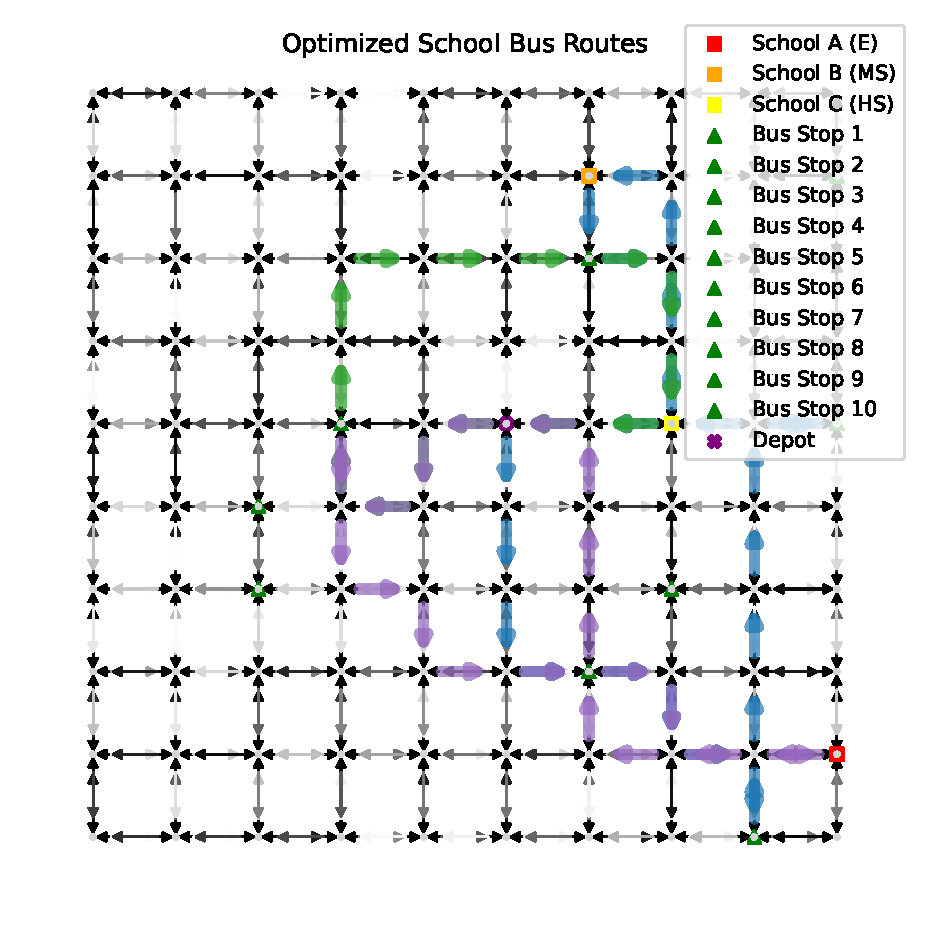
\includegraphics[width=0.5\linewidth, alt={Grid-based toy street network showing optimized school bus routes. Colored route segments connect selected stops to schools and a depot, demonstrating that the routing formulation can generate feasible bus paths on a small artificial network.}]{figures/initial_test.pdf}
    \caption{Initial test of bus routing in a 10 by 10 toy network, using 3 schools of different types, 1 central depot, and 10 total bus stops. Each directed edge has a random weight assigned.}
    \label{fig:placeholder}
\end{figure}

The co-design composition enables a clear separation between physical and institutional subsystems while maintaining their properties. For example, a fleet component maps a set of buses B with capacities $C_b$, ranges $R_b$, and accessibility attributes $W_b$ to feasible routing capabilities. Meanwhile, a staffing component models the availability of monitors and drivers, and a policy component encodes equity goals such as sufficient coverage for particular demographic groups. These components are combined into a global design problem whose solution set can be projected onto different objective spaces like cost, coverage, and equity to generate explicit Pareto frontiers that planners and stakeholders can interrogate.

\section{Data Sources and Preprocessing}

I utilize network, operational, demand, and demographic information and format it into a common mathematical representation. The physical road network is obtained from \gls{osm} and converted into a directed graph $G=\langle V,E,\omega\rangle$, where nodes $V$ represent intersections, depots, stops, and schools. Directed edges $E$ capture feasible roadway movements with associated attributes $\omega_e$ such as length, speed, and travel time. From this base graph, I identify the subset of nodes corresponding to bus pick-up locations $P$, destination locations $S$, and bus depot locations $D$ using geocoded address records and provided facility data.

\gls{gtfs} data can provide scheduled trip patterns, stop locations, and route identifiers for the existing network, which are linked to \gls{osm}-derived nodes. If available, \gls{avl} traces that are representative of a given area are cleaned and matched to the road network to estimate real-world travel times. These estimates are then aggregated for every edge and time-of-day and used to define the travel-time component of $\omega_e$.

Demand is represented as a set of individuals $M$, each associated with a pickup stop $p_m\in P$, an assigned destination $s_m\in S$. For the case study, I additionally employ a school type $\tau_m\in T$ that encodes whether a school is elementary, middle, or high school. Additionally, one can exclude students that reside within a fixed walking threshold $\gamma$ of their destination school by computing network shortest-path distances from each school to nearby residential locations and filtering those below $\gamma$. Demographic attributes from the \gls{acs}, such as income distribution, race and ethnicity composition, English proficiency, and car access, are joined to student and stop nodes via census block groups, which can later be used as equity indicators when evaluating Pareto-optimal designs. 

I also incorporate student-level flags indicating the need for additional on-board support and wheelchair accessibility. A binary flag $f_m$ identifies students in set $F\subseteq M$ who require a monitor, and a subset $W\subseteq F$ identifies those who require a wheelchair-accessible bus. These attributes are derived from the district's special education transportation records and are used to enforce monitor and vehicle constraints at the routing stage. 

\section{Co-Design and \Glsentryfull{milp} Formulation}

\begin{figure}[!htbp]
    \centering
    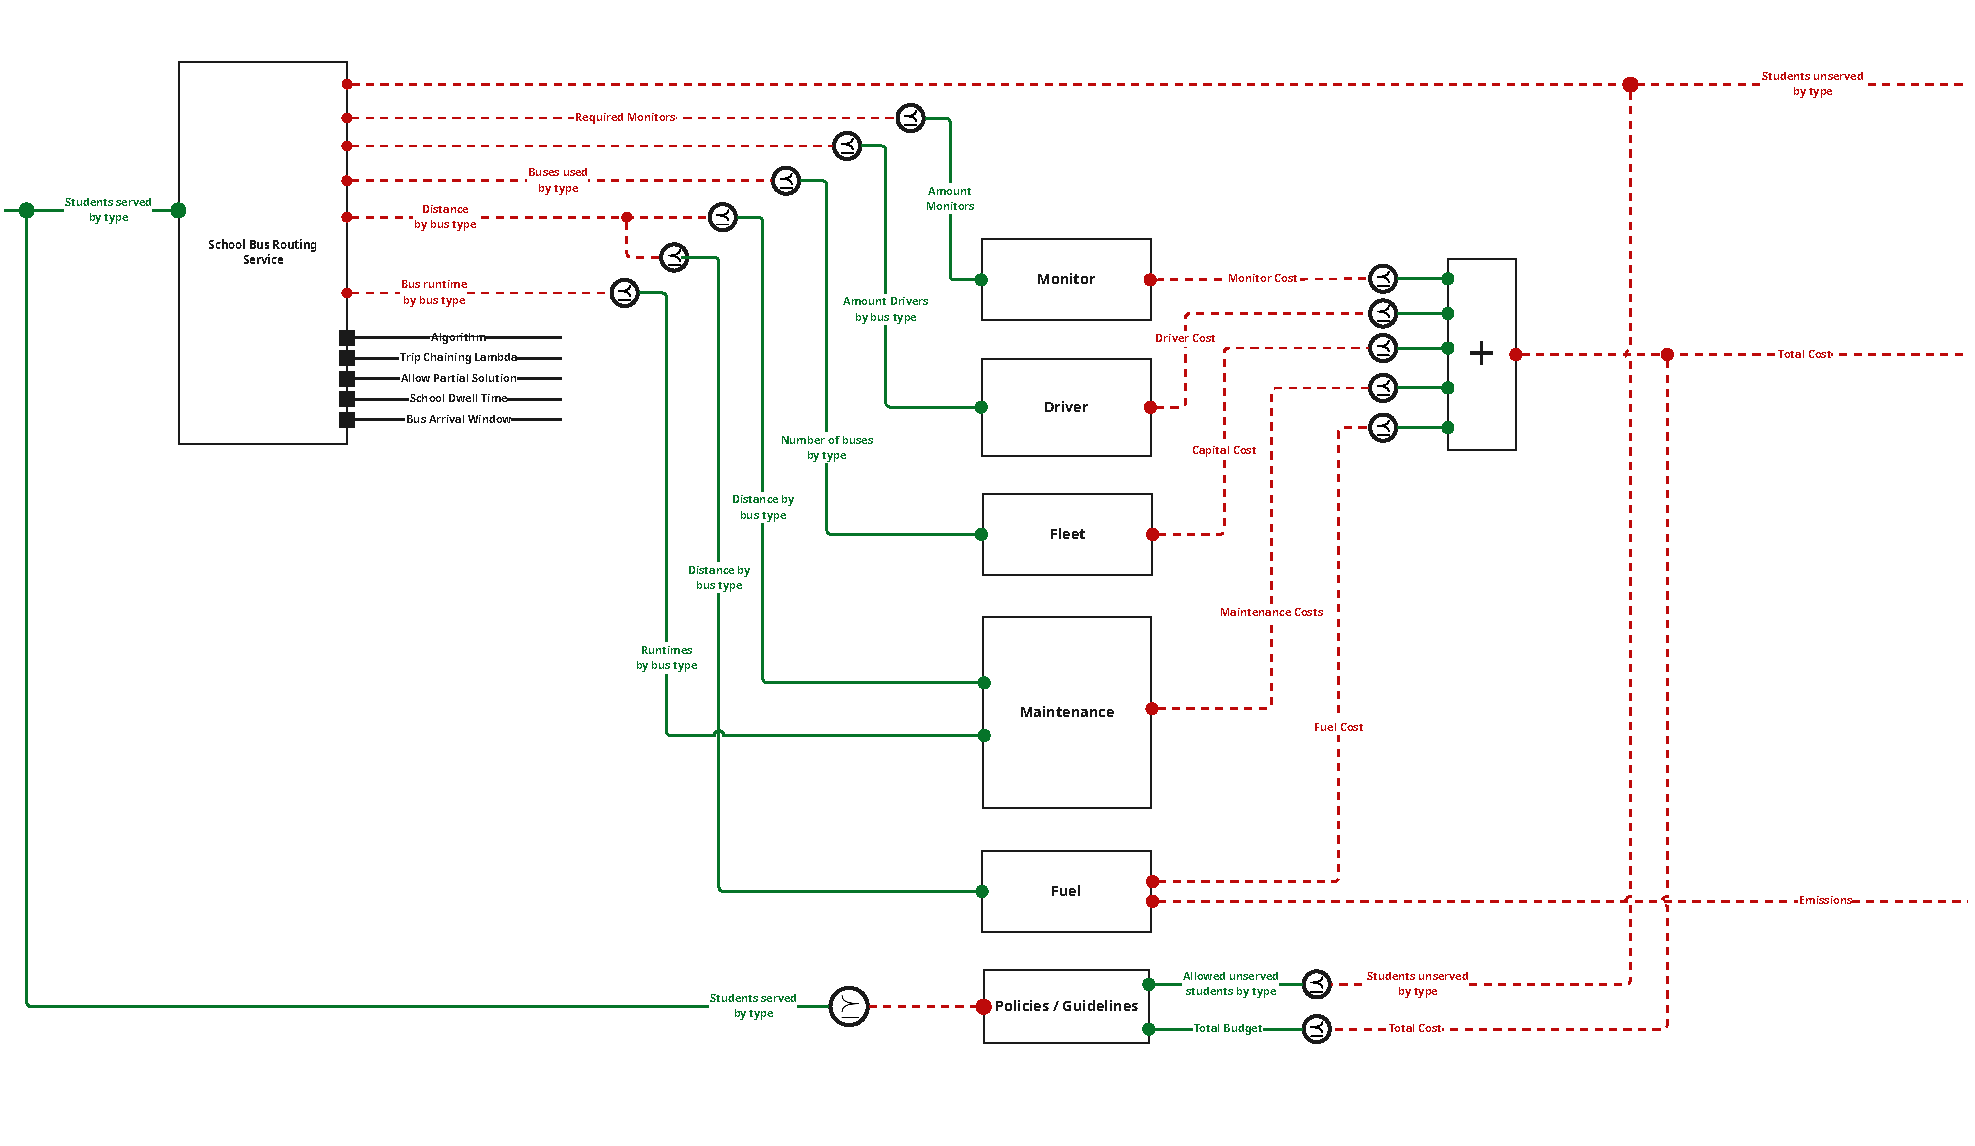
\includegraphics[width=0.99\linewidth, alt={Co-design system diagram showing how routing service inputs, bus capacity, driver, fuel, maintenance, monitor, and \glsentryfull{BiRD} algorithm parameters connect to outputs such as total cost, unserved students, stops used, emissions, and accessibility-related service metrics.}]{figures/codesign_diagram_simple.pdf}
    \caption{Simplified co-design diagram, illustrating how different component functionalities and requirements interact.}
    \label{fig:codesign}
\end{figure}

\autoref{fig:codesign} summarizes the resulting co-design composition, with each box representing an \gls{mdpi} (monitor, bus capacity, driver, fuel, maintenance, and routing service) connected via shared functionalities and resources. At the core of this framework is a decomposed \gls{milp} formulation that encodes the routing and assignment decisions. This can be tailored to a specific use case, and below is a formulation for the specific Framingham case study. The full, original formulation below is presented as background motivation; due to computational intensity, the implementation that follows uses a modified \gls{bird} backend from \textcite{delarueOptimizing}, referred to here as \gls{bra}, with two modes: \verb!scenario! and \verb!lbh!.

\subsection{Initial Formulation}
\label{sec:original_milp}

The routing network is defined by routing nodes $N\coloneqq P\cup S\cup D^{+}\cup D^{-}\cup S^{+}$ and directed arcs $A\subseteq N\times N$, where each arc $(i,j)\in A$ represents travel along a (precomputed) shortest path in $G$ with distance $d_{ij}$ and travel time $t_{ij}$. To model multi-round ``trip chaining'' for each bus, I introduce a set of rounds $Q={1,\ldots,Q_{max}}$, where each round represents a sub-tour that begins at a node and ends either at a school or at the depot. This can be used to reflect a ``multi-tiered'' trip system, while ensuring that the initial round must begin at the depot and the final round must end at the depot.

Decision variables in the \gls{milp} include $z_b$ for whether bus $b$ is used, $z_{b,q}$ for whether bus $b$ operates in round $q$, and $x_{b,q,ij}$ for whether bus $b$ traverses arc $\left(i,j\right)$ in round $q$. The variables $v_{b,q,i}$ are introduced to indicate whether node $i$ is visited by bus $b$ in round $q$, and $e_{b,q,s}$ record whether round $q$ for bus $b$ ends at school $s$, enabling trip chaining via school start-copy nodes $s^{+}$ for subsequent rounds. Student bus assignments are represented by $a_{m,b,q}$, which equals 1 if student $m$ is on bus $b$ in round $q$. These variables enforce that each student is assigned to at most one bus and one round and that all students are served when the coverage ratio $\phi$ is set to 1.

Time and capacity constraints are captured using continuous variables $T_{b,q,i}$ for the arrival time of bus $b$ at node $i$ in round $q$, and integer variables $L_{b,q,i}$ for the on-board passenger load immediately after visiting node $i$. Alighting and boarding service times are set through user defined constant parameters $\alpha=0.3$ minutes per boarding and $\beta=0.5$ minutes per alighting, which both contribute additively to the time-linking constraints on arcs and to the chaining of rounds at schools. To handle differences in school types and bus capacity for different ages, the \gls{milp} formulation also includes binary variables $y_{b,q,\tau}$ specifying the active school type $\tau\in T$ for each bus and round, along with a multiplier $\kappa_\tau$ that scales the functional capacity of bus $b$ according to the served school type (e.g. elementary school students can fit 3 to a seat compared to 2 for middle and high schoolers).

The objective function minimizes a weighted sum of total distance traveled across buses, an optional per-round tiebreaker, and an indicator for using buses with monitors (which increases labor cost). Specifically, the primary term sums distances $d_{ij}$ over all active arcs $x_{b,q,ij}$, while a small penalty $\lambda_{\mathrm{round}}$ is applied to $z_{b,q}$ to discourage unnecessary tour fragments (without overriding distance minimization when $\lambda_{\mathrm{round}}$ is small). An additional term $r_b^{\mathrm{mon}}$ indicates whether bus $b$ carries a monitor, which allows the optimization to incorporate monitor staffing costs or prioritize configurations that reduce monitor deployment (while still meeting all special transportation constraints) by summing across all buses.

These constraints together enforce student assignment coverage, tour feasibility, time consistency, max time limits, capacity adherence, and monitor and wheelchair-accessibility requirements. Assignment constraints ensure each student is assigned at most once and that the aggregate number of assigned students meets the desired coverage $\phi\left\vert M\right\vert$. Flow-conservation and depot/school connection constraints also ensure that each round is a valid tour.

Time-linking constraints guarantee that arrival times along arcs respect travel plus dwell times and that buses depart schools for the next round only after boarding/alighting. Latest-arrival constraints require that the arrival time at each school $s$, plus the relevant alighting dwell, does not exceed the latest allowable arrival $\ell_s\coloneq h_s-\delta_s$, where $h_s$ is the bell time (represented as minutes from midnight) and $\delta_s$ is a required slack. To control individual student experiences, precedence constraints enforce that a student’s school is visited after their pickup stop by at least a small separation $\epsilon$, and ride-time constraints require that the difference $T_{b,q,s_m}-T_{b,q,p_m}$ does not exceed an arbitrary maximum in-vehicle time $H_{\mathrm{ride}}$ when $a_{m,b,q}=1$.

Capacity dynamics are handled by linking the load variables $L_{b,q,i}$ across arcs by using the number of students boarding or alighting at each node and bounding the load by the actual capacity $C_b\sum_{\tau}\kappa_\tau y_{b,q,\tau}$. Additional constraints set loads to zero at depots and school start-copy nodes to reset tours, as well as ensure that ending a round at a school implies an empty bus at that school (if required). Monitor-related constraints couple the presence of flagged students $m\in F$ with the binary variable $r_b^{\mathrm{mon}}$, making sure that any bus carrying a flagged student in any round also carries a monitor, and also that wheelchair-using students $m\in W$ can only be assigned to buses with $W_b=1$.

\begin{figure}[!htbp]
    \centering
    \begin{subfigure}{0.495\textwidth}
        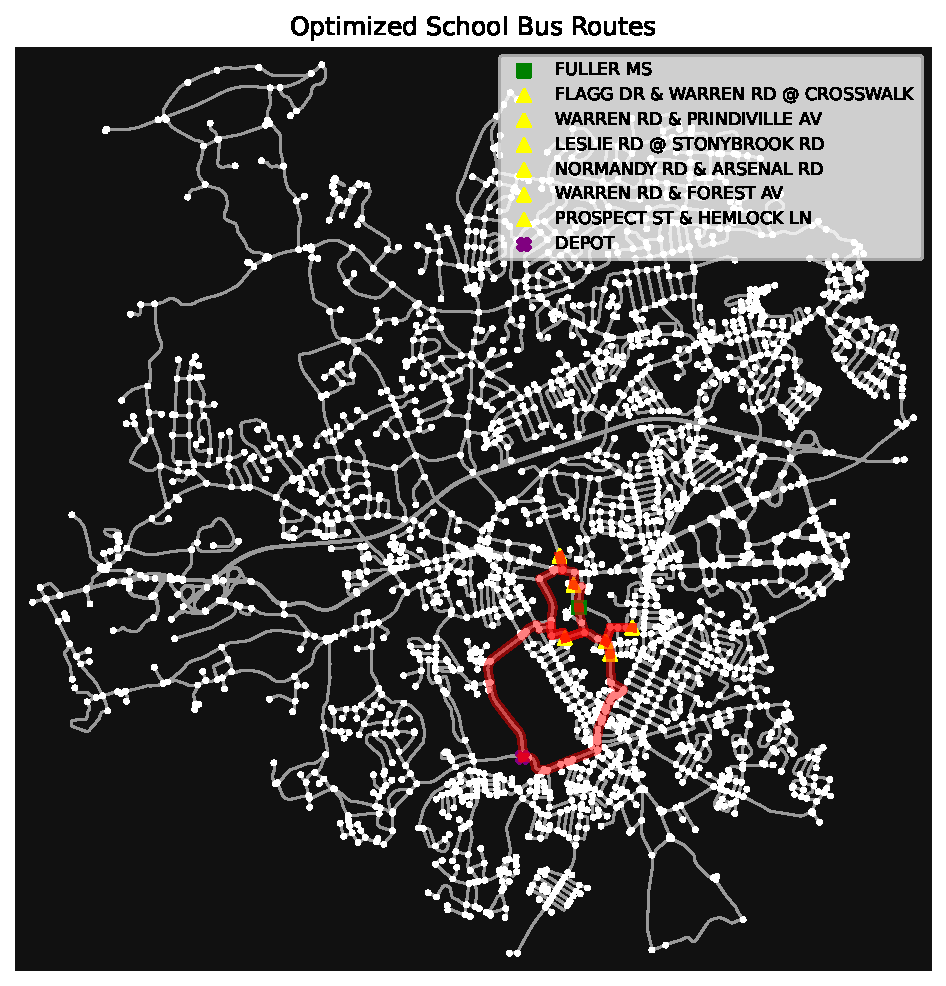
\includegraphics[width=0.99\textwidth, alt={Map of initial optimized bus routes for students within one kilometer of a school, without trip chaining. Red route segments show the selected bus path over the Framingham road network.}]{figures/no_chaining_routes.pdf}
        \subcaption{All students within 1 km of a school (no chaining)}
    \end{subfigure}
    \begin{subfigure}{0.495\textwidth}
        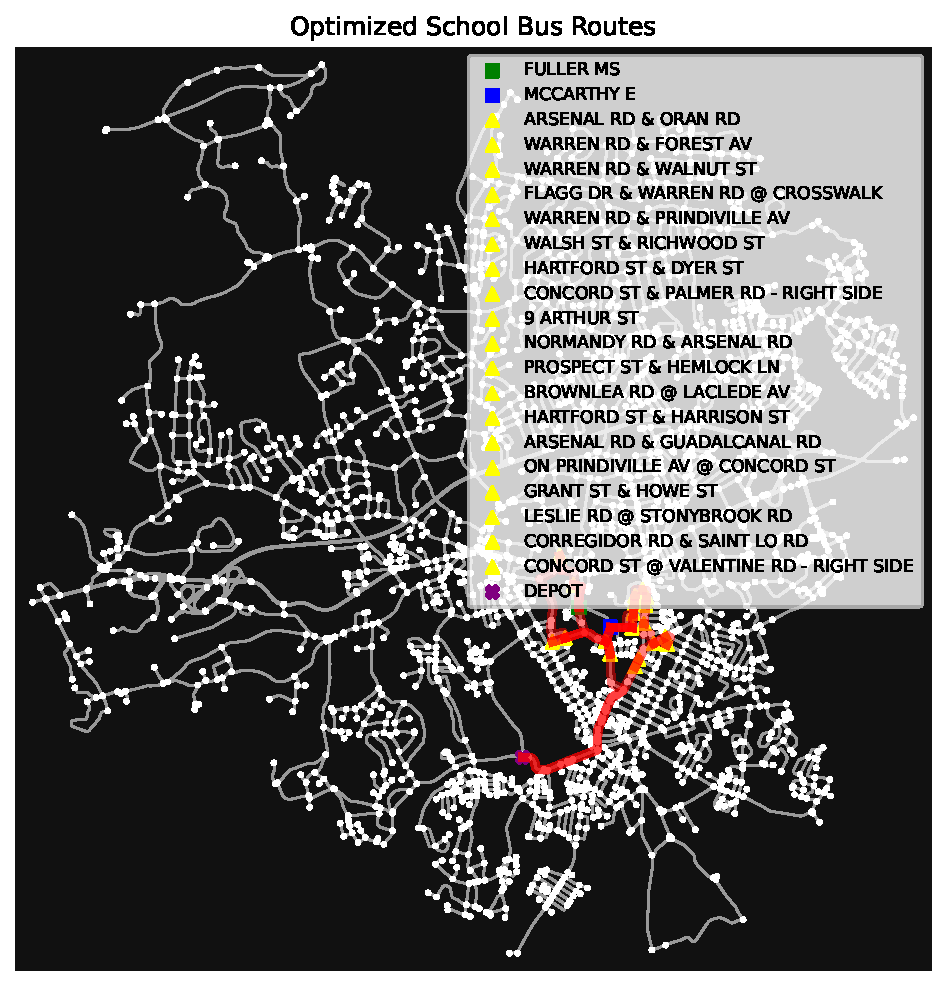
\includegraphics[width=0.99\textwidth, alt={Map of initial optimized bus routes for students within one kilometer of two schools, with trip chaining. Red route segments show the selected bus path over the Framingham road network.}]{figures/chaining_routes.pdf}
        \subcaption{All students within 1 km of 2 schools (chaining)}
    \end{subfigure}
    \caption{Initial test routes using the original formulation}
    \label{fig:prelim_results}
\end{figure}

Informally, the \gls{milp} chooses which buses to use, what arcs they traverse, and which students they carry, while simultaneously respecting capacity, maximum ride time, and school arrival windows. It does all this while also attempting to minimize a weighted sum of distances and bus/monitor usage. While this was able to handle small networks well as shown in \autoref{fig:prelim_results}, this became computationally prohibitively expensive as the problem size increased. 

\subsection{\Glsentryfull{bird} Backend Formulation}

The implemented \gls{bird} backend provides two main routing algorithms: a scenario-based optimization method and a constructive \gls{lbh}, denoted as \verb!scenario! and \verb!lbh!. Both methods operate on the same underlying  representation, which stores schools, stops, student assignments, fleet attributes, travel times, bell times, and special transportation requirements. However, they differ in how they search the feasible design space.

The \verb!scenario! method follows a generate-and-optimize structure. First, it constructs a large pool of feasible candidate routes using greedy nearest-insertion procedures under multiple different parameter settings. These configurations are the ``scenarios'' in the implementation: alternative route-generation settings used to vary the candidate pool. Each candidate route serves a single school $s$ and already satisfies local feasibility constraints such as vehicle capacity, school arrival timing, student ride-time limits, and special transportation restrictions. The second stage then solves a \gls{milp} that selects from this candidate set. In the homogeneous case, this resembles a set-covering formulation in which binary route-selection variables cover required stops while minimizing a weighted route cost. In the fleet-aware case, the model additionally assigns selected routes to specific buses, tracks bus usage, and permits chaining multiple school routes onto a single vehicle when the resulting arrival and departure times remain feasible.

The fleet-aware \verb!scenario! formulation is therefore a decomposed alternative to the full arc-based \gls{milp} described in \autoref{sec:original_milp}. Rather than deciding every street-level arc traversal directly, it optimizes over complete feasible route candidates. The model includes variables indicating whether a bus is used, whether a route is assigned to a bus, whether a route begins or ends a bus itinerary, and whether two routes can be linked consecutively by the same bus. Sparse linking variables encode only temporally feasible route-to-route transitions, reducing the number of impossible chaining decisions considered by the solver. The implementation also solves the problem in service groups, routing wheelchair-accessible students first, then students requiring transportation with staff monitors, and finally students without additional transportation needs. This structure reflects operational priority constraints, while still allowing later stages to use remaining fleet capacity.

The \verb!lbh! method provides a faster solver-free baseline. Instead of generating many routes and solving a mixed-integer selection problem, it constructs bus itineraries directly through repeated cheapest insertion. Buses are considered in capacity-priority order, and the algorithm inserts uncovered stops into the current itinerary whenever doing so preserves capacity, grade compatibility, maximum ride-time, and school timing feasibility. For fixed bell-time schools, insertions are evaluated against a fixed arrival constraint; for schools with allowable time windows, the insertion logic also accounts for the flexibility of the arrival window. As in the scenario-based method, the fleet-aware heuristic proceeds through wheelchair, monitor-required, and conventional service groups.

These two \gls{bird} modes expose a useful quality-runtime tradeoff. The \verb!scenario! method is slower and requires a \gls{milp} solver, but it can make globally coordinated decisions over a diverse pool of candidate routes and explicitly optimize route chaining across a heterogeneous fleet. The \verb!lbh! method is substantially faster and does not require a solver, but it makes locally optimal decisions: once a stop insertion or bus assignment is made, the algorithm does not globally reconsider that choice. In the framework, \verb!scenario! is therefore used when higher-quality optimized designs are desired, while \verb!lbh! provides a computationally lightweight benchmark and fallback routing procedure. Pareto fronts created using this method and testing data can be seen in \autoref{fig:bird_simple}.

\begin{figure}[!htbp]
    \centering
    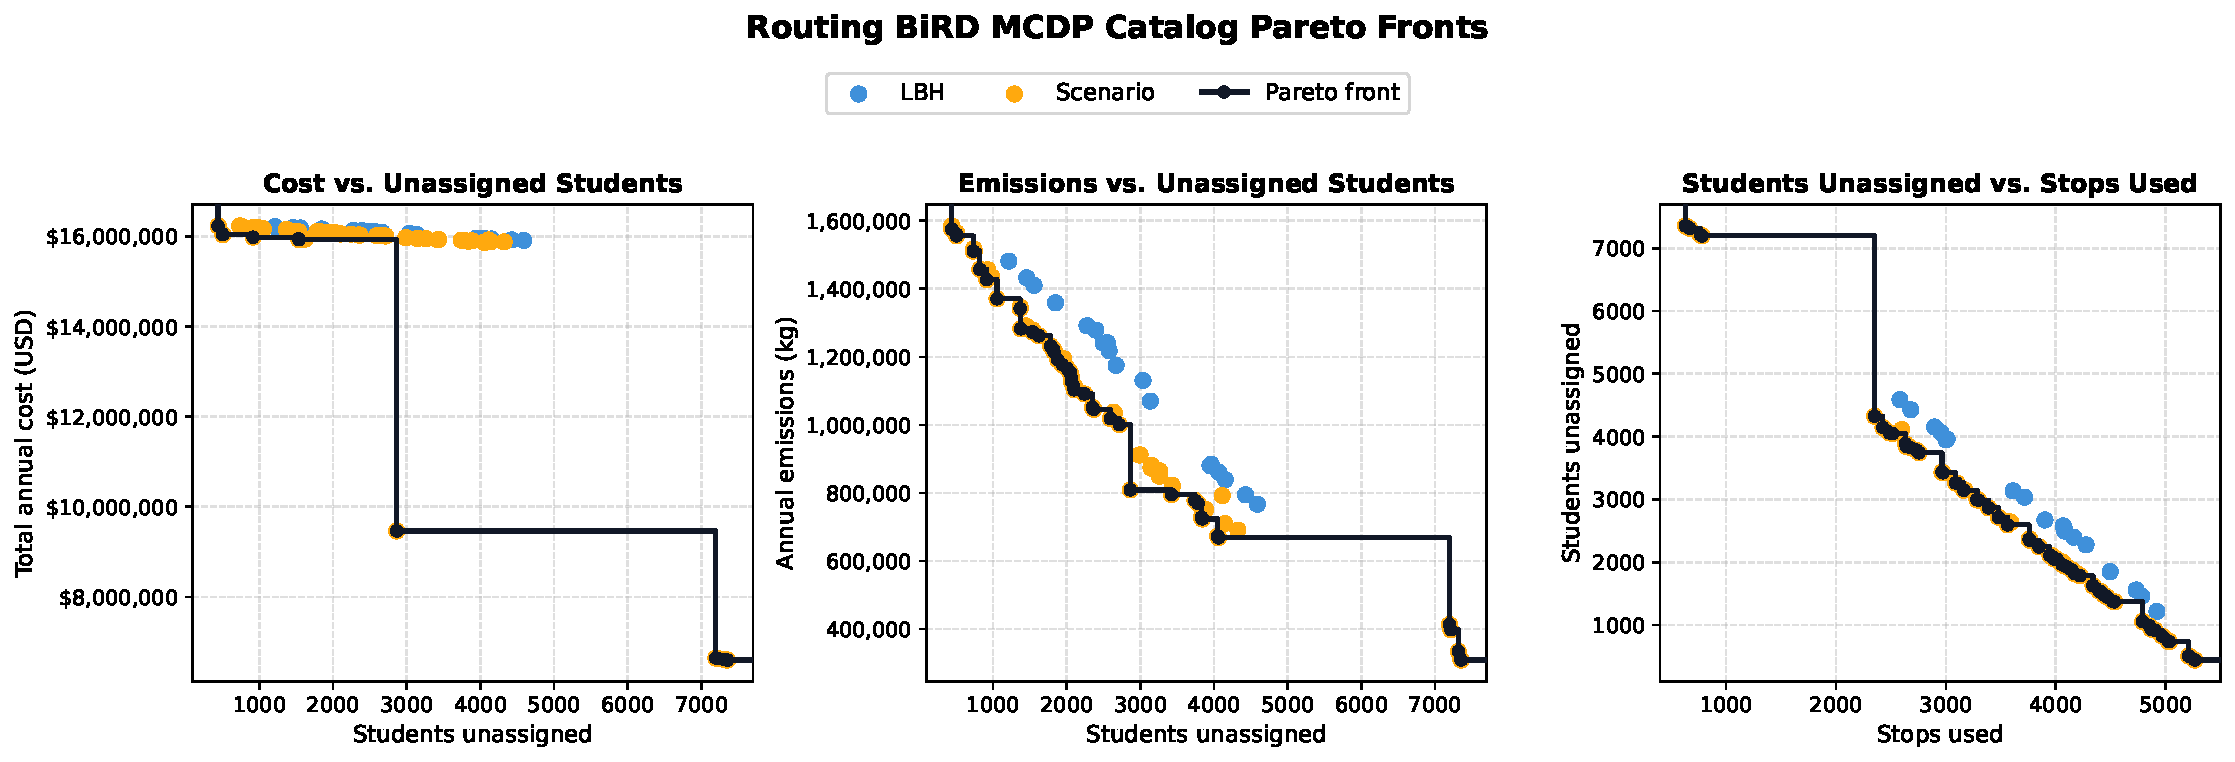
\includegraphics[width=0.99\linewidth, alt={Three side-by-side Pareto-front scatter plots comparing \glsentryfull{lbh} and Scenario \glsentryfull{bird} outputs on catalog data. The plots show tradeoffs between unassigned students and cost, unassigned students and annual emissions, and stops used and cost. Blue points represent \glsentryfull{lbh} solutions, red points represent scenario solutions, and the black line marks the Pareto frontier.}]{figures/routing_bird_mcdp_pareto_all.pdf}
    \caption{Pareto fronts using \gls{bird} with all possible different configurations.}
    \label{fig:bird_simple}
\end{figure}

\section{Case Study Implementation for Framingham}

I implement the framework described for the Framingham, Massachusetts school bus system to illustrate its practical use in evaluating and redesigning a real-world network. The case study for \gls{fps} focuses on morning school arrivals for a single day representative of regular operations, using district-provided data on student assignments, current route structures, fleet composition, and special transportation requirements. Thus, I map the provided data into the sets and parameters for \gls{bra}, including the actual fleet $B$, depot configuration $D$, school set $S$, and student set $M$ with flags $F$ and $W$, and use the candidate-route selection and decomposition model. The \gls{osm}-derived Framingham road network used to construct travel arcs is shown in \autoref{fig:framingham}.

\begin{figure}[!htbp]
    \centering
    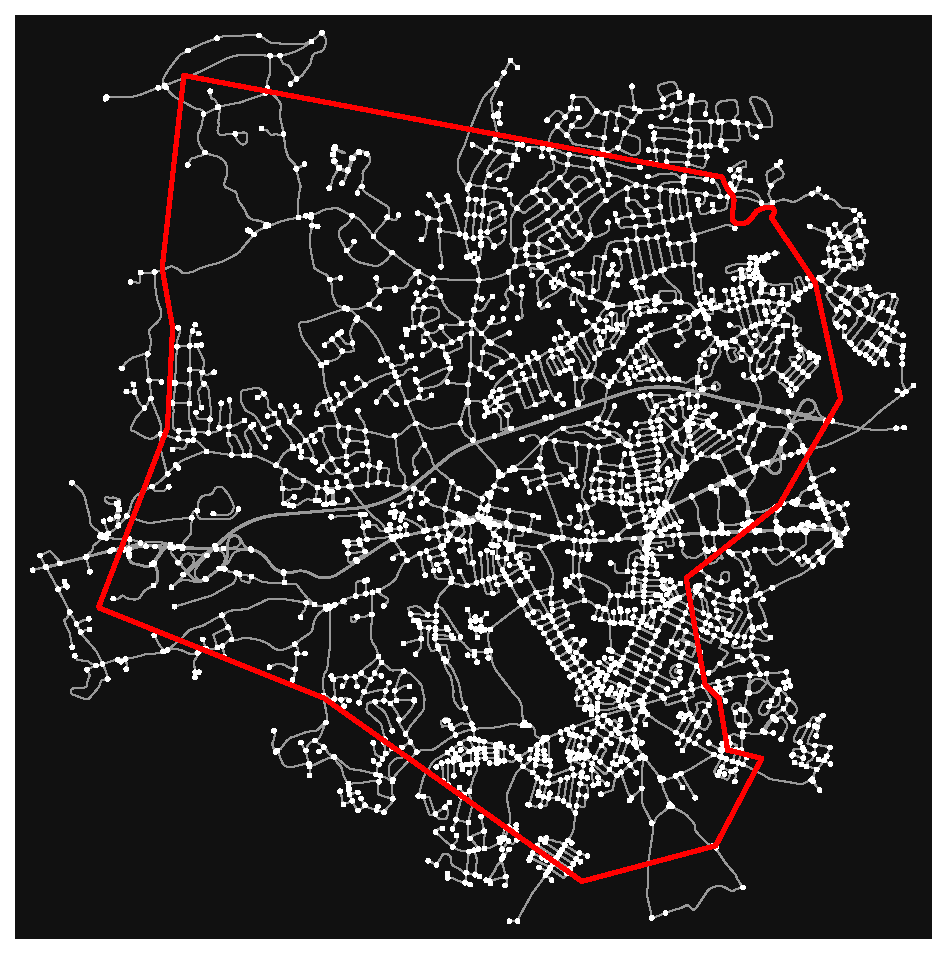
\includegraphics[width=0.5\linewidth, alt={Map of the Framingham road network used to construct travel arcs. White road segments appear on a dark background, with a red boundary outlining the study area.}]{figures/framingham.pdf}
    \caption{Current Framingham road network used to create travel arcs}
    \label{fig:framingham}
\end{figure}

To implement this for Framingham, I first encoded the current routing pattern directly into the same format used in \gls{bird}, allowing comparisons between existing routes with generated ones. This produces a feasible design point in the co-design framework that reflects the existing system. I then solve the \gls{bird} candidate-selection model under the same resource constraints but with different objective weightings to generate a family of alternative feasible designs.

I also explore multiple values of $Q_{max}$ to allow or restrict the extent of trip chaining and examine how this affects fleet utilization and student ride times. Furthermore, one can use a $Q_{max}$ of 1 to determine whether trip chaining is beneficial. To investigate equity outcomes, I compute post-solution metrics such as coverage rates by income quintile, average and maximum ride times by demographic group, and the spatial distribution of unassigned or long-ride students relative to \gls{acs}-based vulnerability indices.

The categorical co-design framing shaped the Framingham experiments by treating routing as a compositional feasibility problem: district resources, service requirements, accessibility constraints, and environmental costs are modeled as interconnected design variables rather than as a single monolithic objective. The Pareto fronts therefore represent the feasible tradeoff surface exposed by this design space, showing how changes in one component, such as fleet use, stop coverage, or student service, propagate through the broader transportation system.

\section{Extension to Urban Bus Network Redesigns}

Although this thesis focuses on a case study for school bus operations in Framingham, Massachusetts, the underlying co-design framework is intended to generalize to urban bus networks more broadly. The same monotone composition of physical, operational, and policy subsystems applies when planners restructure bus routes, frequencies, and stop patterns across all-day service.

In an urban transit context, several modeling elements change, while the overall structure stays intact. To begin, the demand representation would typically shift from discrete student assignments to a continuous or aggregated demand model, such as \gls{od} matrices, time-of-day boarding patterns, or stop-level ridership patterns. Rather than assigning individual students $m\in M$ to specific trips, the framework should be modified to embed demand as flows along corridors or between urban activity centers, which can then feed into \gls{mdpi} components that evaluate coverage and travel time distributions for different rider populations.

In addition, stop placement and spacing become explicit design variables, rather than fixed inputs. In this school bus case study, pickup locations are predetermined by student addresses and district policies, and the road network is treated as a base on which to route vehicles. For cities, the co-design problem can include a stop-setting component that trades off walk access distance, stop spacing, and in-vehicle travel time. This would allow the framework to represent both ``coverage-orientation'' and ``frequency-oriented'' network designs, all with the same formalism.

Furthermore, the temporal structure must expand from single-trip or peak-period service to all-day (and potentially weekend) operations. Instead of enforcing arrival windows around school start and end times, an urban setting would require time-dependent headways, service distribution, and coordination between routes at transfer points. These considerations can be captured by extending the temporal \gls{mdpi} components to include time-of-day frequency decisions and reliability metrics, composing them with fleet and crew scheduling components to model multi-shift operations.

Equity objectives must also shift, from school-specific ride times and eligibility thresholds to accessibility and service quality across diverse neighborhoods and rider groups. The same co-design framework can incorporate equity metrics based on job accessibility, access to healthcare and other key destinations, as well as by implementing constraints on headways, crowding, or travel time disparities between demographic or income groups. In this way, the framework is highly adaptable, providing a unified and formal language for representing a wide variety of transportation planning problems, the main differences residing in how demand, stop placements, temporal patterns, and equity indicators are instantiated and resolved within the shared structure.

\chapter{Results}
\label{ch:results}

\Gls{fps} provided the core datasets required to conduct a preliminary routing analysis: school locations, schools served, school start times, student home locations, assigned schools, grade levels, current bus assignment, and fleet characteristics, including bus size, capacity, and type. \gls{fps} also confirmed that all buses operate from a single central depot and that current school transportation is planned independently of the local public transportation provider, \gls{mwrta}. Accordingly, \gls{mwrta} service is excluded from this analysis.

The available data is sufficient to identify and assess the current routing and test alternative configurations, but it is not yet sufficient for final implementation. The key limitation is that the dataset for currently served students includes assigned stops and disability status, but these records cannot be directly linked to each student's home address. This prevents full validation of current stop assignments and limits the precision of student-level service comparisons. I estimate Census-based demographic information by determining the corresponding block-group for different student addresses, then randomly sampling based on the percentage returned from \gls{acs} 5-year estimates.

\begin{table}[!htbp]
    \centering
    \begin{tabular}{@{}lll@{}}
    \toprule
        Category & Quantity & Avg Dist. to School [mi] \\ \midrule
        All students in \gls{fps} & 8210 & 2.81 \\
        Students currently riding bus & 4780 & 3.55 \\
        Within 1 mile of school & 1085 & 0.62 \\
        Within 2 miles of school & 2412 & 1.35 \\
        Further than 5 miles from school & 531 & 5.36 \\
        Language other than English at home & 4034 & 2.97 \\
        Non-car owning household & 760 & 3.03 \\
        Students with disabilities & 1096 & 2.49 \\ 
        \bottomrule
    \end{tabular}
    \caption{\gls{fps} student demographics and average home-to-school distance by student group, reported in miles. Categories are not mutually exclusive; a student may belong to multiple rows.}
    \label{tab:demographics}
\end{table}

\section{Existing Routes}
\label{sec:existing_routes}

Current routing is shaped by the interaction between district school choice policies and Massachusetts transportation requirements. Under Massachusetts General Laws (MGL Ch. 71, Section 68), districts must provide free transportation to K-6 students living more than 2 miles from school. As shown in \autoref{fig:geospatial}, this policy creates a clear incentive for some families in Framingham to select schools farther from home in order to secure transportation coverage. This pattern is especially visible among lower-income and minority households in the southern part of the city, as well as among families of students with disabilities.

\begin{figure}[!htbp]
    \centering
    \begin{subfigure}{0.33\textwidth}
        \subcaption{Students by distance to school}
        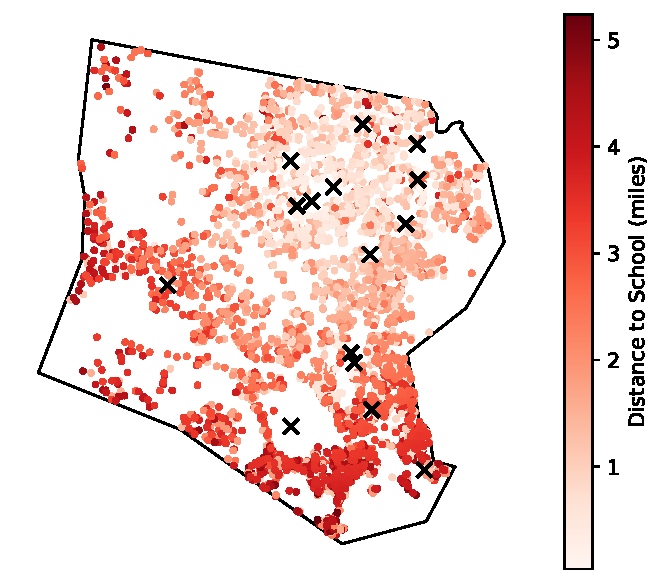
\includegraphics[width=0.99\textwidth, alt={Map of student locations in Framingham colored by distance to school. Darker red points indicate students farther from school, with schools marked by black X symbols.}]{figures/students_distance_to_school.pdf}
    \end{subfigure}
    \begin{subfigure}{0.33\textwidth}
        \subcaption{Location of students with disabilities}
        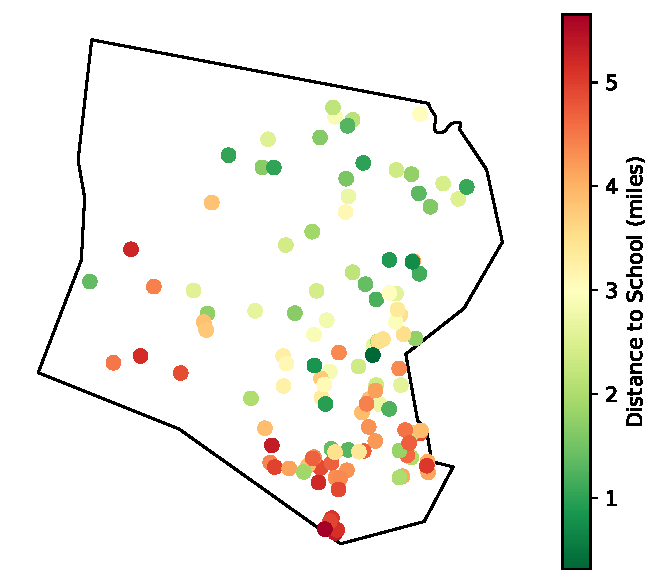
\includegraphics[width=0.99\textwidth, alt={Map of students with disabilities in Framingham colored by distance to school. Points show student locations, and warmer colors indicate longer school distances.}]{figures/special_education_students.pdf}
    \end{subfigure}
    \begin{subfigure}{0.33\textwidth}
        \subcaption{Median income by block group}
        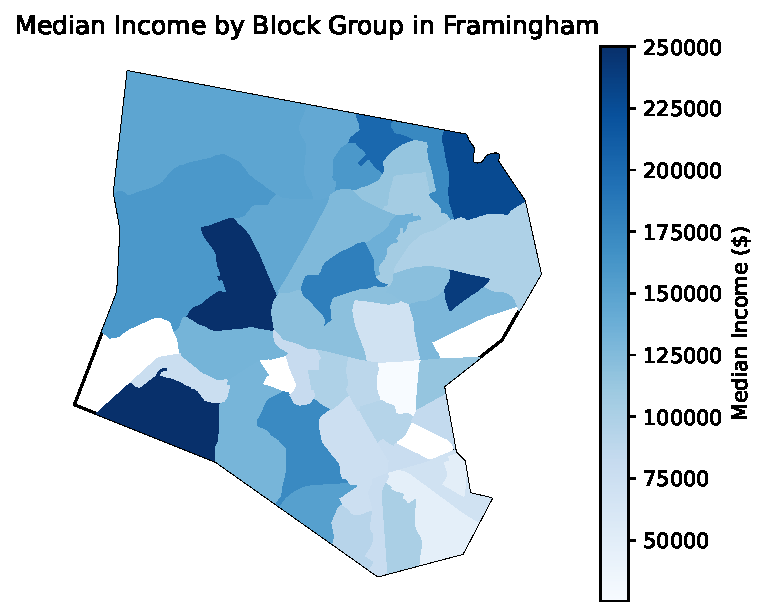
\includegraphics[width=0.99\textwidth, alt={Choropleth map of median income by census block group in Framingham. Darker blue areas indicate higher median income, and lighter areas indicate lower median income.}]{figures/median_income_by_block_group.pdf}
    \end{subfigure}
    \caption{Plots of different socioeconomic factors in Framingham, MA. Block groups from U.S. Census 2020.}
    \label{fig:geospatial}
\end{figure}

The current assignment therefore reflects both operational routing decisions and upstream policy-driven demand. At present, \gls{fps} uses 51 buses (with a maximum of 86 available) to serve 219 students with disabilities and 4,561 students without disabilities at the identified schools (4,780 riders total, matching \autoref{tab:demographics}).

\section{Experimental Methodology}

I use \gls{osm} to model the road network and connect it with existing depot, stop, and school locations. Based on walking distances computed using \textcite{fink2022R5py}, students are assigned to their closest stops (or for currently served students, impose the current assignment). Given the available bus fleet, school bell/start times, a manually set time window before these bell times, and a maximum in-vehicle ride-time (here set to 60 minutes), I then compute new routes based on the described \gls{bra}, adapting the decomposition approach of \textcite{bertsimasOptimizingSchoolsStart2019}. 

Because \gls{fps} was not yet able to provide real-world \gls{avl} data, \gls{bra} assumes a fixed driving speed of 30 miles per hour, incorporating boarding and alighting times of the various student groups (including students with disabilities, students requiring wheelchair-accessible routes, and students without additional transportation needs), and allows for multiple rounds by the same bus, dropping off students at one school before picking up additional students and bringing them to another school. To do so, this approach first allocates routes to students requiring accessible routes and students with disabilities, then caters to the remaining students.

\section{Currently Assigned Students}

The preliminary results indicate that \gls{bra} can improve \gls{fps}'s bus operations while preserving student coverage. Under the tested configuration, the algorithm serves the same 4,780 currently assigned students using 48 buses instead of 51, reducing deployed buses by 3, or approximately 5.9\%. This suggests that the existing network contains meaningful routing inefficiency that can be addressed through algorithmic reassignment and multi-school bus utilization. The core operational advantage of \gls{bra} is that it allows each bus to complete multiple trips across schools, while each trip remains structured around a specific grade and school assignment. For this preliminary test, I use conservative estimates and assume buses travel at an average speed of 30 miles per hour, require 30 seconds for student boarding, 1 minute for boarding students with disabilities, arrive between 10 minutes and 40 minutes before school bell time, and include a required 10-minute dwell time at the school as a buffer.

\begin{table}[!htbp]
    \centering
    \begin{tabular}{@{}lllllllll@{}}
        \toprule
        Category 
        & \multicolumn{4}{l}{\textbf{Current Routing}} 
        & \multicolumn{4}{l}{\textbf{BRA with Current Students}} \\
        & Mean & StDev & Min & Max 
        & Mean & StDev & Min & Max \\ 
        \midrule
        Currently assigned 
        & 43.08 & 29.00 & 3.05 & 133.38 
        & 30.52 & 14.13 & 1.64 & 58.31 \\
        Non-English at home 
        & 41.24 & 28.16 & 3.91 & 133.38 
        & 31.18 & 13.72 & 1.64 & 58.31 \\
        Non-car owning household 
        & 39.83 & 27.89 & 3.91 & 133.37 
        & 30.66 & 13.28 & 1.64 & 58.23 \\
        Students with disabilities
        & 36.68 & 20.82 & 3.05 & 125.38 
        & 25.35 & 13.33 & 2.14 & 57.86 \\
        \midrule
        Buses used 
        & \multicolumn{4}{l}{51} 
        & \multicolumn{4}{l}{48} \\
        \bottomrule
    \end{tabular}
    \caption{Estimated travel times in minutes for currently assigned riders under current routing versus the \gls{bra} configuration. Does not account for intersection delay, assumes constant bus speed.}
    \label{tab:travel_times}
\end{table}

The benefits are not limited to fleet utilization. Across all tracked student groups, \gls{bra} reduces estimated mean travel times relative to the current routing baseline, as shown in \autoref{tab:travel_times}. For currently assigned bus riders, mean travel time falls from 43.08 minutes to 30.52 minutes, a reduction of approximately 29.2\%, while the maximum observed travel time falls from 133.38 minutes to 58.31 minutes. 

Vulnerable groups also see consistent improvements under the modeling assumptions (\autoref{tab:travel_times}): mean travel time declines from 41.24 to 31.18 minutes for students from households where English is not the primary language, from 39.83 to 30.66 minutes for students from non-car-owning households, and from 36.68 to 25.35 minutes for students with disabilities. Additionally, because mean travel time decreased for non-car-owning households by approximately 23.0\% under \gls{bra}, this suggests that efficiency improvements are not achieved by sacrificing service to transit-dependent households. \autoref{fig:routes} shows the current and proposed route layouts side-by-side.

These findings are directional rather than final, since the analysis does not yet account for intersection delay, time-varying congestion, or all student-specific service requirements (e.g. wheelchair students due to missing data). Nonetheless, they establish a clear proof of concept: better route design can potentially allow \gls{fps} to serve the same students with fewer buses, shorter rides, and more consistent travel times across demographic groups.

\section{All Students}

\begin{figure}[!htbp]
    \centering
    \begin{subfigure}{0.32\textwidth}
        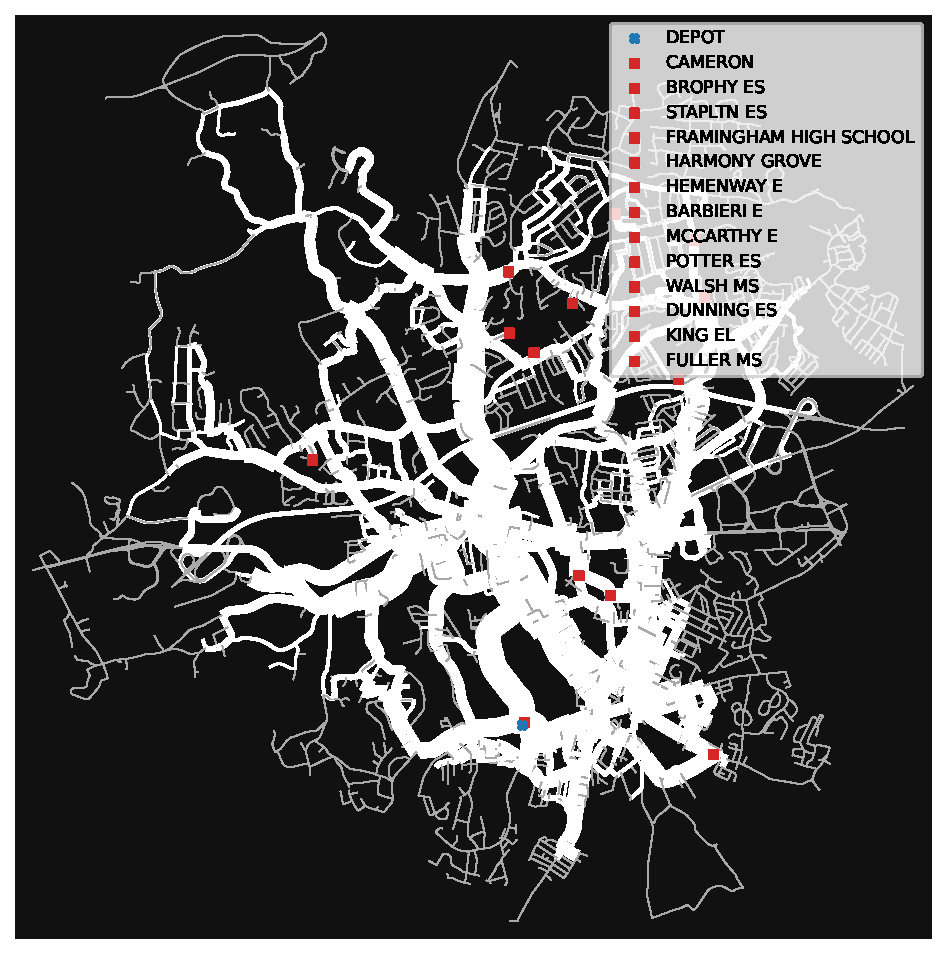
\includegraphics[width=0.99\textwidth, alt={Route-density map of current \glsfullentry{fps} bus routes. White road links indicate roads used by more buses, with selected route segments highlighted in red.}]{figures/existing_routes.pdf}
        \subcaption{Current routes used by \gls{fps}}
    \end{subfigure}
    \begin{subfigure}{0.32\textwidth}
        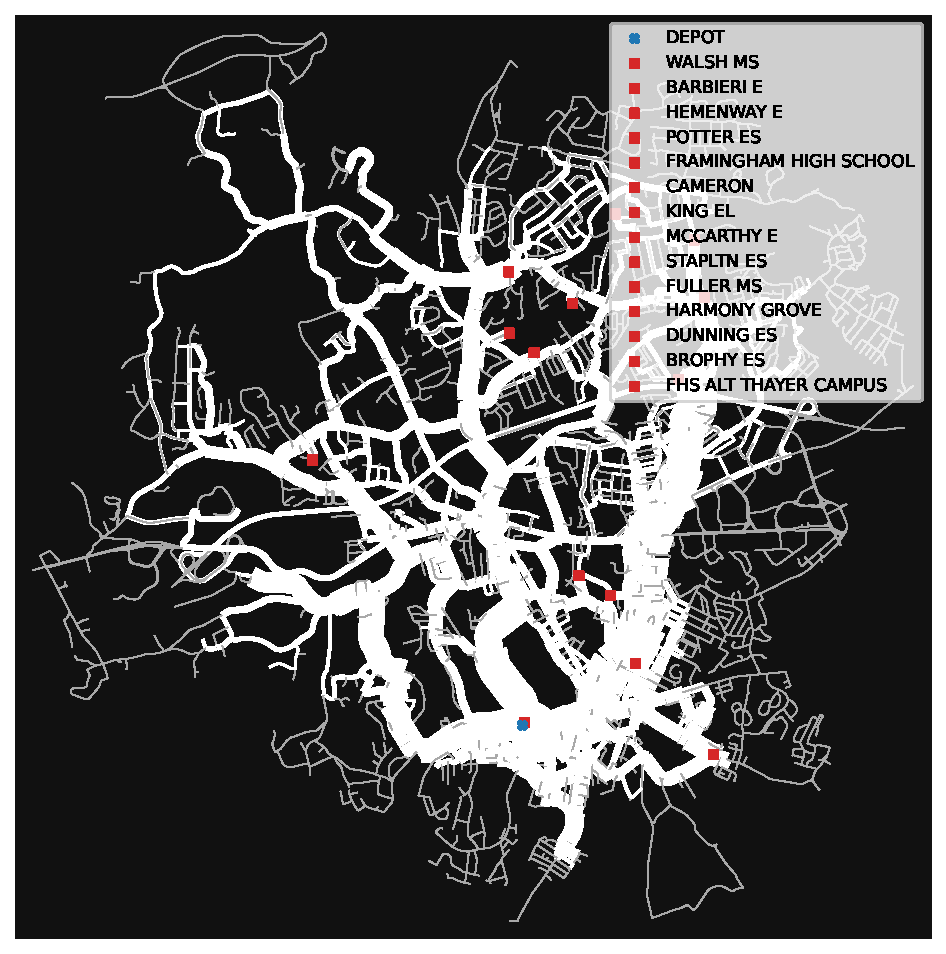
\includegraphics[width=0.99\textwidth, alt={Route-density map of proposed routes generated using \glsfullentry{bra}. White road links indicate roads used by more buses, with selected route segments highlighted in red.}]{figures/bird_assigned_students_routes.pdf}
        \subcaption{Proposed routes generated using \gls{bra}}
    \end{subfigure}
    \begin{subfigure}{0.32\textwidth}
        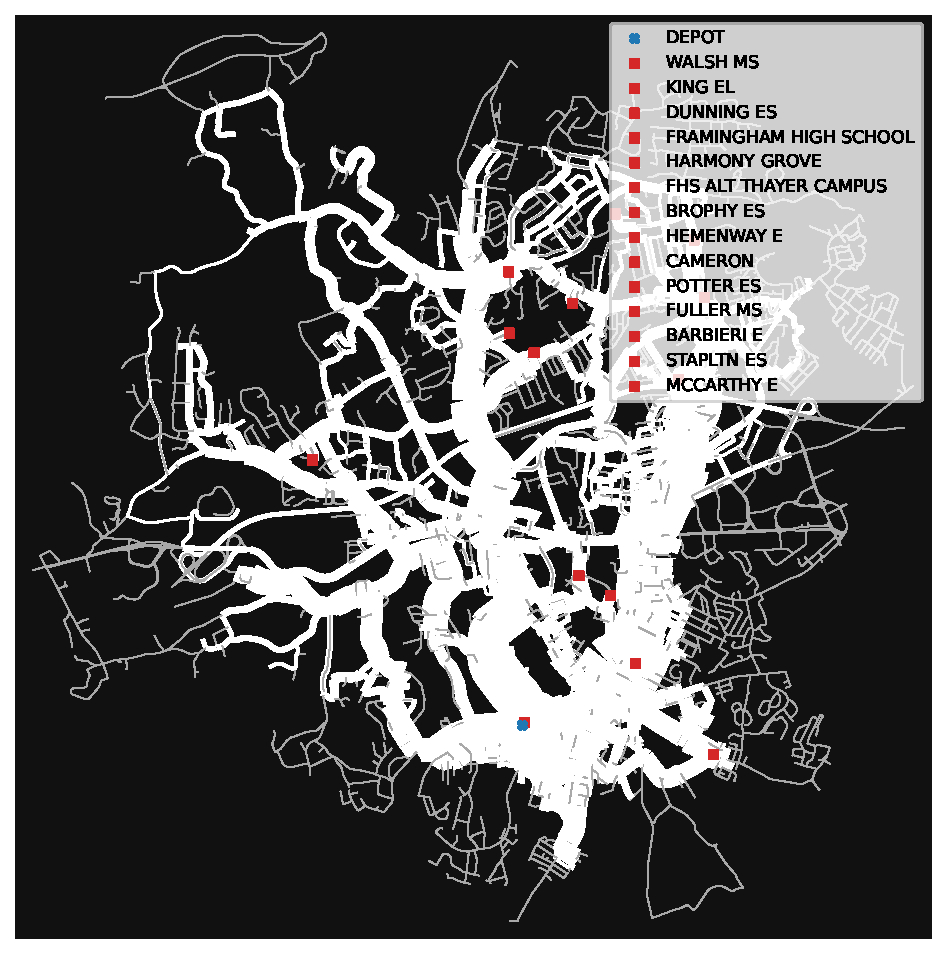
\includegraphics[width=0.99\textwidth, alt={Route-density map of possible routing for students at least 1.5 miles from school. White road links indicate roads used by more buses, with selected route segments highlighted in red.}]{figures/bird_all_students_over_1_5_miles.pdf}
        \subcaption{Possible routing of students $\geq$ 1.5 miles away}
    \end{subfigure}
    \caption{Visualization of routes, with each road link represented by how many buses travel along it.}
    \label{fig:routes}
\end{figure}

Additionally, \gls{fps} is moving from an opt-in routing model to an opt-out model, where students are provided transport by default. Thus, I applied \gls{bra} with the current fleet constraints and found that the current student population living over 1.5 miles\footnote{As mentioned in \autoref{sec:existing_routes}, \gls{fps} is required under Massachusetts law to offer no-cost transportation for students living over 2 miles away. However, as of writing, \gls{fps} also offers bus transportation for students living between 1 and 2 miles away for an associated fee \cite{framinghampublicschoolsRider, framinghamschoolcommittee2022Student}.} from their school can be served using the existing fleet available to \gls{fps}. Conversely, all students in the district with the current bus fleet cannot be fully served with the assumed modeling and operational constraints, as shown in \autoref{tab:travel_times_all}. While these preliminary results are directional and should be further refined, they demonstrate how \gls{fps} can substantially change their bus routing to serve a greater number of students while improving average travel-time outcomes under the modeled assumptions.

\begin{table}[!htbp]
    \centering
    \begin{tabular}{@{}lllllllll@{}}
        \toprule
         Served & \multicolumn{4}{l}{\textbf{All Students $\geq$ 1.5 miles away}} & \multicolumn{4}{l}{\textbf{All students}} \\
         & Mean & StDev & Min & Max & Mean & StDev & Min & Max \\ \midrule
         All students 
         & 30.81 & 14.67 & 3.52 & 59.62 
         & 29.67 & 14.95 & 0.73 & 59.76 \\
         Non-English at home 
         & 31.69 & 14.49 & 3.55 & 59.62 
         & 30.77 & 14.47 & 0.73 & 59.43 \\
         Non-car owning household 
         & 32.24 & 14.00 & 4.60 & 59.62 
         & 31.68 & 14.41 & 2.41 & 59.76 \\
         Students with disabilities 
         & 29.93 & 14.37 & 4.55 & 58.26 
         & 30.52 & 15.03 & 2.14 & 59.76
         \\ \midrule 
         Total number of students & \multicolumn{4}{l}{6304} & \multicolumn{4}{l}{8210} \\
         Students unassigned & \multicolumn{4}{l}{0} & \multicolumn{4}{l}{13} \\ 
         Buses used & \multicolumn{4}{l}{62} & \multicolumn{4}{l}{78} \\
         \bottomrule
    \end{tabular}
    \caption{Estimated travel times of students in minutes with different routing configurations with the set of all students. Does not account for intersection delay, assumes constant bus speed.}
    \label{tab:travel_times_all}
\end{table}

The Pareto fronts in \autoref{fig:pareto} summarize the tradeoffs induced by varying resource limits and objective weights in the \gls{bra} candidate-selection model. Each point represents a feasible routing configuration generated under the same data assumptions but with different priorities over fleet use, coverage, and student travel time. I also analyze the current \gls{fps} routing plan as a baseline design, making it easy to assess whether existing operations are dominated by generated alternatives under the modeled constraints. Because travel times are estimated using simplified speed assumptions rather than calibrated \gls{avl} data, these fronts should be interpreted as relative planning comparisons rather than final operational schedules.

\begin{figure}[!htbp]
    \centering
    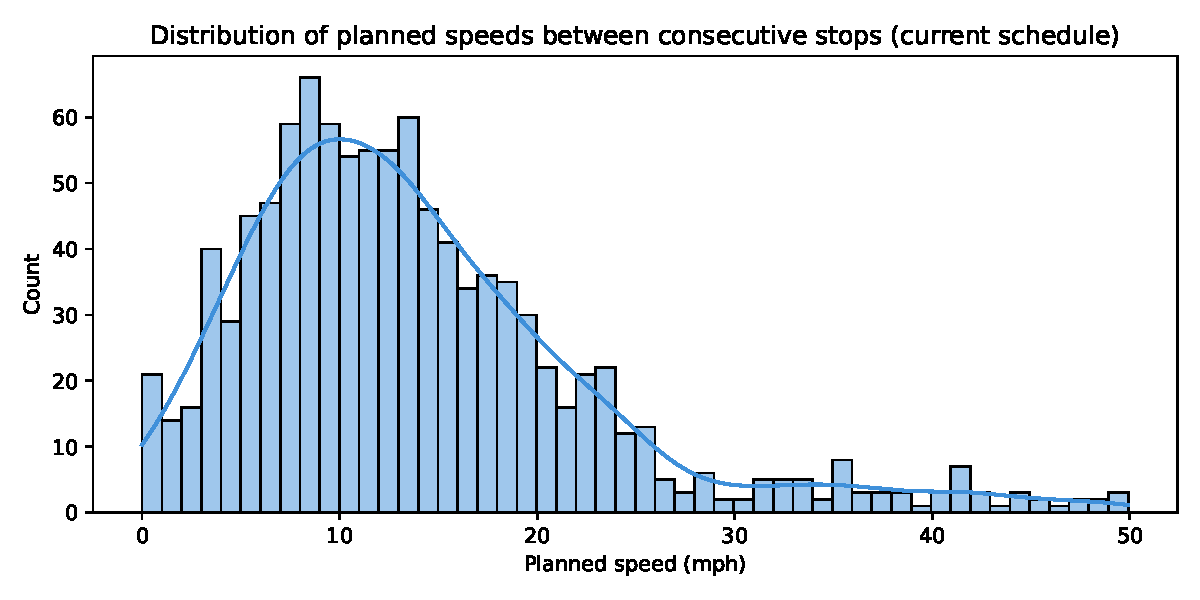
\includegraphics[width=0.99\textwidth, alt={Histogram of implied planned bus speeds between consecutive stops, measured in kilometers per hour. Most stop-to-stop segments fall between about 5 and 20 km/h, with the highest concentration around 10 to 15 km/h and a long right tail extending toward 50 km/h, indicating substantial variation in planned travel speeds.}]{figures/current_schedule_speed_distribution.pdf}
    \caption{Distribution of implied planned speeds between consecutive stops in the existing route data. Speeds are calculated from planned stop-to-stop movements and show substantial variation across route segments.}
    \label{fig:planned-speed-distribution}
\end{figure}

Although the \gls{bra} experiments use a constant-speed assumption for travel-time estimation, the existing route data suggest that planned bus speeds vary substantially across stop-to-stop segments. \autoref{fig:planned-speed-distribution} shows that most implied planned speeds are well below free-flow arterial speeds, with a long right tail of faster segments. This reinforces that the results should be interpreted as comparative planning estimates rather than deployment-ready schedules, and that future work should calibrate travel times using \gls{avl} traces or a time-dependent routing engine.

\begin{figure}[!htbp]
    \centering
    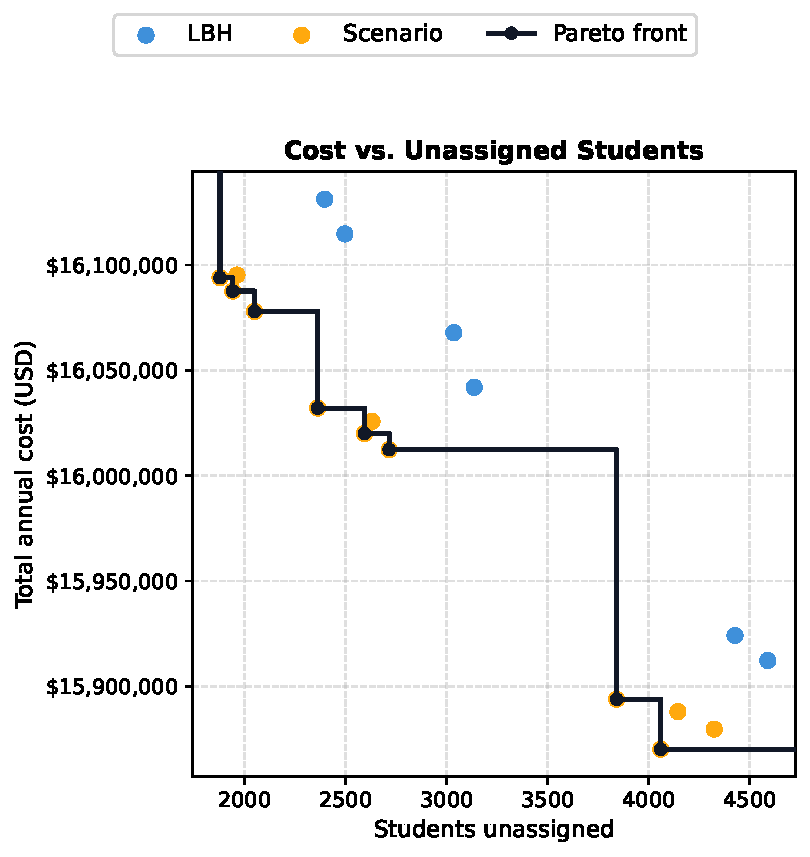
\includegraphics[width=0.495\linewidth, alt={Scatter plot of total annual cost versus students assigned for \glsfullentry{bird} testing data. \glsfullentry{lbh} and Scenario solutions are plotted to compare how stop usage affects cost.}]{figures/routing_bird_mcdp_pareto_routing_simple_caps_cost_unassigned.pdf}
    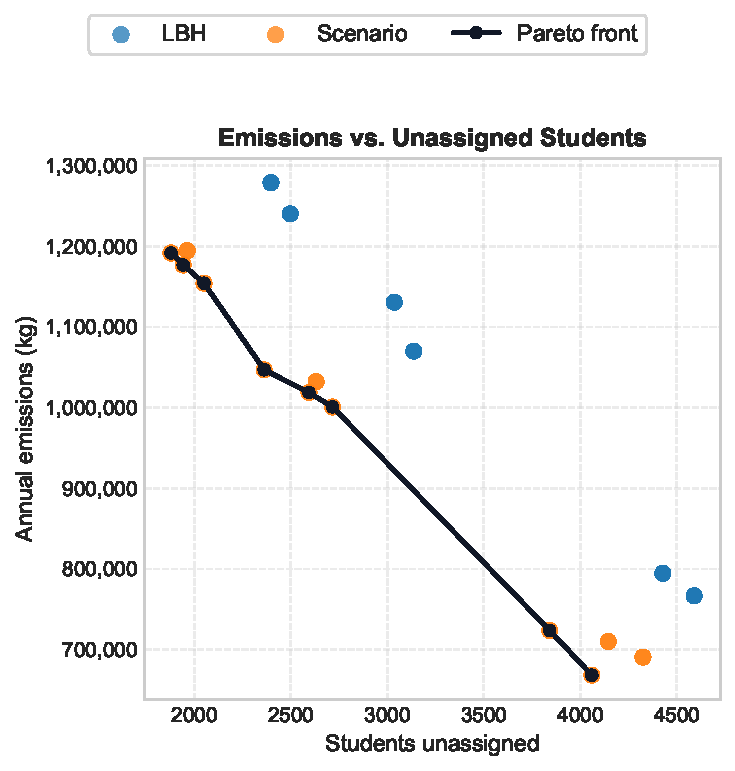
\includegraphics[width=0.495\linewidth, alt={Scatter plot of total annual cost versus students assigned for \glsfullentry{bird} testing data. \glsfullentry{lbh} and Scenario solutions are plotted, with the Pareto frontier showing the best emission-coverage tradeoff.}]{figures/routing_bird_mcdp_pareto_routing_simple_caps_emissions_unassigned.pdf}
    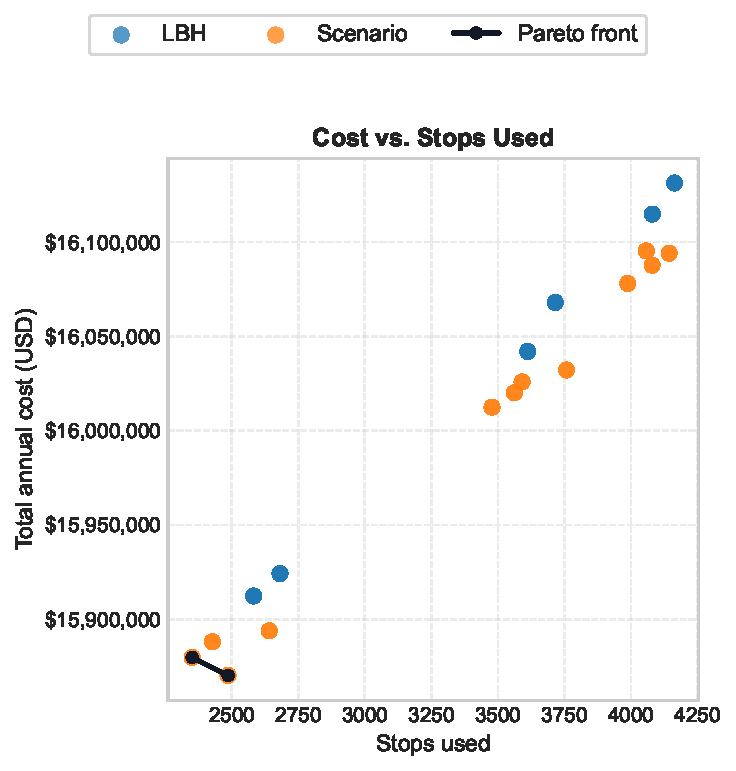
\includegraphics[width=0.495\linewidth, alt={Scatter plot of total annual cost versus students assigned for \glsfullentry{bird} testing data. \glsfullentry{lbh} and Scenario solutions are plotted, with the Pareto frontier showing the best cost-coverage tradeoff.}]{figures/routing_bird_mcdp_pareto_routing_simple_caps_cost_stops.pdf}
    \caption{Pareto fronts for \gls{bra} simplified routing configuration with student data. Each point on these fronts is a valid solution of the co‑design problem with different resource allocations among \gls{mdpi} components (fleet, driver, monitor, fuel, maintenance). The figure makes visible the planning tradeoffs implied by the categorical composition.}
    \label{fig:pareto}
\end{figure}

To refine these results further, future work will require \gls{fps} to provide a unified student-level dataset linking each student's home location, school, grade, transportation eligibility, current stop assignment, bus assignment, disability status, wheelchair-accessibility requirement where applicable, and any district-specific service constraints. Additionally, I would like to confirm whether routing should use district-approved stops or allow \gls{bra} to generate new stop assignments, and also whether demographic equity constraints should be embedded directly into the \gls{bra} optimization using a strategy similar to \textcite{paviaDesigningEquitableTransit2023}.

As this work is continued, one should define service standards that should govern implementation, including maximum ride time, maximum walk distance to stops, arrival windows, and treatment of students with disabilities and accessibility needs. Future work should replace constant-speed assumptions with calibrated travel times that reflect road type, congestion, and school-period traffic conditions.

\chapter{Discussion and Limitations}

These findings are directional rather than final, since the analysis does not yet account for intersection delay, time-varying congestion, or all student-specific service requirements (e.g. wheelchair students due to missing data). Nonetheless, they establish a clear proof of concept: better route design can potentially allow \gls{fps} to serve the same students with fewer buses, shorter rides, and more consistent travel times across demographic groups. Additionally, they demonstrate how \gls{fps} can substantially change their bus routing to serve a greater number of students while improving average travel-time outcomes under the modeled assumptions.

To refine these results further, future work will require \gls{fps} to provide a unified student-level dataset linking each student's home location, school, grade, transportation eligibility, current stop assignment, bus assignment, disability status, wheelchair-accessibility requirement where applicable, and any district-specific service constraints. Additionally, I would like to confirm whether routing should use district-approved stops or allow \gls{bra} to generate new stop assignments, and also whether demographic equity constraints should be embedded directly into the \gls{bra} optimization using a strategy similar to \textcite{paviaDesigningEquitableTransit2023}.

As this work is continued, one should define service standards that should govern implementation, including maximum ride time, maximum walk distance to stops, arrival windows, and treatment of students with disabilities and accessibility needs. Future work should replace constant-speed assumptions with calibrated travel times that reflect road type, congestion, and school-period traffic conditions.

\section{Extension to Urban Bus Network Redesigns}

This thesis focuses on a case study for school bus operations in Framingham, Massachusetts, but the underlying co-design technique can be generalized to urban bus networks more broadly. The same monotone compositional reasoning of physical, operational, and policy subsystems applies when planners restructure bus routes, frequencies, and stop patterns across all-day service.

In an urban transit context, several modeling elements change, while the overall structure stays intact. To begin, the demand representation would shift from discrete student assignments to a model of passenger demand, such as \gls{od} matrices, time-of-day boarding patterns, or stop-level ridership patterns. Rather than assigning individual students $m\in\mathcal{M}$ to specific trips, one should embed demand as flows along corridors or between urban activity centers, which can then feed into \gls{mdpi} components that evaluate coverage and travel time distributions for different rider populations.

In addition, stop placement and spacing become explicit design variables, rather than fixed inputs. In this school bus case study, pickup locations are predetermined by student addresses and district policies, and the road network is treated as a base on which to route vehicles. For cities, the co-design problem can include a stop-setting component that trades off walk access distance, stop spacing, and in-vehicle travel time. This would allow one to represent both ``coverage-orientation'' and ``frequency-oriented'' network designs, all with the same formalism.

Furthermore, the temporal structure must expand from single-trip or peak-period service to all-day (and potentially weekend) operations. Instead of enforcing arrival windows around school start and end times, an urban setting would require time-dependent headways, service distribution, and coordination between routes at transfer points, as well as the consideration of multi-modal alternatives. These considerations can be captured by extending the temporal \gls{mdpi} components to include time-of-day frequency decisions and reliability metrics, composing them with fleet and crew scheduling components to model multi-shift operations, and by composing multiple different components together to represent multi-modal operations (possibly by reusing components).

Equity objectives must also shift, from school-specific ride times and eligibility thresholds to accessibility and service quality across diverse neighborhoods and rider groups. The same co-design framework can incorporate equity metrics based on job accessibility, access to healthcare and other key destinations, as well as by implementing constraints on headways, crowding, or travel time disparities between demographic or income groups. In this way, the framework is highly adaptable, providing a unified and formal language for representing a wide variety of transportation planning problems, the main differences residing in how demand, stop placements, temporal patterns, and equity indicators are instantiated and resolved within the shared structure.
\chapter{Conclusions}
\label{ch:conclusions}

The Framingham case study demonstrates that the \gls{bra} implementation can expose operational tradeoffs that are difficult to see from the existing route plan alone. For the currently assigned bus riders, \gls{bra} serves the same 4,780 students using 48 buses rather than 51, a reduction of 3 buses, or approximately 5.9\%. At the per-bus daily lease cost discussed in \hyperref[ap:stakeholder]{Appendix~\ref*{ap:stakeholder}} (low hundreds of dollars), this corresponds to a meaningful annual lease-cost reduction before accounting for fuel and labor. At the same time, estimated mean travel time falls from 43.08 minutes to 30.52 minutes, and the maximum observed travel time falls from 133.38 minutes to 58.31 minutes. Under the modeled assumptions and conservative operational constraints, this suggests that the current routing pattern is improved upon by feasible alternatives that use fewer vehicles while also reducing student ride times---a more efficient and equitable system.

The all-students experiments show that expanding transportation access creates a different tradeoff. Serving students who live at least 1.5 miles from school is feasible under the modeled assumptions, though closer to the fleet limit. In \autoref{tab:travel_times_all}, the model uses 62 buses for the 1.5-mile eligibility case, leaving no students unassigned under the assumed constraints. When all students are considered, the model serves a larger total population but leaves 13 students unassigned, indicating that universal default service is not achievable without either additional resources, relaxed service standards, revised stop assignment rules, or a different policy definition of eligibility.

These results also illustrate the value of the Pareto-front framing. Rather than producing a single ``best'' routing plan, the co-design formulation can show the frontier between competing objectives. This is useful for planning because the preferred solution may depend on institutional priorities: one configuration may minimize buses, another maximizes student coverage, and another could reduce long rides for vulnerable groups. By placing the current \gls{fps} routing plan on the same frontier as generated alternatives, the framework allows planners to distinguish between tradeoffs that are structurally unavoidable and inefficiencies that can be improved through redesign.

Equity considerations are central to this interpretation. The results show that students from non-English-speaking households, non-car-owning households, and students with disabilities all experience lower estimated mean travel times under \gls{bra} than under the current routing baseline. This suggests that efficiency improvements do not come at the expense of vulnerable groups. However, the current experiments evaluate equity primarily after routing, rather than embedding equity constraints directly in the optimization objective. Future versions should incorporate explicit constraints or penalties for unequal service outcomes, such as subgroup-specific maximum ride times, minimum coverage rates, or limits on the spatial concentration of unassigned students. Additionally, inspired by the work of \textcite{vanweeEvaluatingTransportEquity2021}, promising outcomes could be gained by identifying ways of indexing inequity levels and incorporating them into \gls{bra}.

The results should therefore be interpreted as planning evidence rather than deployment-ready schedules. The current model assumes a constant travel speed, does not include intersection delay or time-varying congestion, and lacks complete student-level linkage between home addresses, current stops, bus assignments, disability status, and wheelchair-accessibility requirements. These limitations affect the precision of individual travel-time estimates and may change which route chains are feasible in practice. Before implementation, the model should be recalibrated using district-validated stop assignments, complete accessibility data, and travel-time estimates derived from \gls{avl} data or a time-dependent routing engine.

Overall, the case study supports the central claim of this work: a co-design-based routing framework can help districts reason about bus network redesign under multiple objectives. \Gls{bra} provides a practical backend for generating feasible routing alternatives, while the Pareto-front representation clarifies how operational efficiency, coverage expansion, and equity goals interact. For \gls{fps}, the preliminary results indicate that meaningful improvements may be possible, particularly for currently assigned riders, but that broader opt-out service requires explicit policy choices about eligibility thresholds, fleet deployment, maximum ride times, and equity guarantees.

Taken together, this thesis contributes a compositional framework (grounded in the monotone co-design theory of \textcite{censi2016Mathematical}) for analyzing school bus routing as a co-design problem rather than a standalone vehicle-routing task. The \gls{mdpi} decomposition (fleet, monitor, driver, fuel, maintenance, and routing service components composed via shared functionality/resource interfaces, as in \autoref{fig:codesign}) is what enables planners to vary one component at a time and analyze the resulting Pareto front, rather than re-solving an entire monolithic \gls{milp} for each scenario. By adapting the \gls{bird} backend into the \gls{bra}, the work connects district resources, service requirements, accessibility needs, emissions, and cost within a single tradeoff-oriented optimization pipeline. The Framingham case study demonstrates that this framework can translate real district data into feasible alternative routing designs and Pareto fronts that make the consequences of different planning priorities explicit. For planners, this enables a more transparent form of analysis: instead of asking only for the lowest-cost routes, districts can evaluate how operational, environmental, and equity objectives interact before selecting routes for further testing or implementation.

\section{Future Work}

Future work should first focus on turning the Framingham case study from a planning proof of concept into an operationally calibrated routing tool. This requires replacing the constant-speed travel-time assumption with travel times derived from \gls{fps} \gls{gps} or \gls{avl} traces, time-dependent routing engines, or both. It also requires a unified student-level dataset that links home location, assigned school, grade, eligibility status, current stop, current bus assignment, monitor requirement, wheelchair-accessibility requirement, and district-specific service constraints under an appropriate privacy agreement. With these data, the model could validate current stop assignments, distinguish between route-level and student-level service changes, and test generated routes with operators before any live deployment.

A second direction is to embed equity more directly into the optimization and co-design layers. The current analysis evaluates subgroup outcomes after routing and shows that estimated mean ride times improve for several vulnerable groups, but it does not yet constrain the optimization to guarantee equitable outcomes. Future versions should incorporate stakeholder-defined equity metrics such as subgroup-specific ride-time ceilings, minimum service coverage, accessibility thresholds, concentration-index penalties, or Rawlsian/leximax objectives. The same framework should also be tested beyond Framingham, both on synthetic benchmark districts and on larger real districts, to evaluate scalability, sensitivity to local policy choices, and the degree to which the co-design representation generalizes from school bus routing to broader urban bus network redesign.


%%% Appendicies of thesis  %%%%%%%%%%%%%%%%%%%%%%%%%%%%%%%%%%%%%%%%%%%%%%%%%%%%%%%%%%%%%%%%%%%%%%%%

\appendix
\include{stakeholder}
\chapter{\Glsentryshort{milp} Representation of \Glsentryshort{bra} Routing Modes}
\label{ap:math}

BRA exposes two routing modes: a scenario-based candidate-selection model and an \gls{lbh} mode. The scenario mode is naturally represented as a \gls{milp} over a generated set of candidate routes. The \gls{lbh} mode is implemented as a constructive insertion heuristic, but it can be interpreted as a greedy approximation to a related bus-itinerary assignment problem.

\section{Scenario Candidate-Selection Formulation}

Let $M$ denote the set of students, $S$ the set of schools, $B$ the set of buses, and $R$ the set of candidate single-school routes generated by the scenario procedure. Each route $r\in R$ serves a subset of students $M_r \subseteq M$, visits a school $s\left(r\right)\in S$, has travel cost $c_r$, travel time $t_r$, and requires a vehicle type compatible with the students assigned to it. Let $a_{m,r}=1$ if student $m$ is served by candidate route $r$, and 0 otherwise. Let $K\subseteq R\times R$ be the set of feasible route links, where $\left(r,r'\right)\in K$ means that the same bus can complete route $r$ and then route $r'$ while respecting school arrival times, deadhead travel time, and required buffer times.

We introduce binary variables
\[
x_r =
\begin{cases}
1 & \text{if route } r \text{ is selected},\\
0 & \text{otherwise,}
\end{cases}
\]
\[
z_b =
\begin{cases}
1 & \text{if bus } b \text{ is used},\\
0 & \text{otherwise,}
\end{cases}
\]
\[
y_{b,r} =
\begin{cases}
1 & \text{if route } r \text{ is assigned to bus } b,\\
0 & \text{otherwise,}
\end{cases}
\]
and
\[
\ell_{b,rr'} =
\begin{cases}
1 & \text{if bus } b \text{ operates route } r' \text{ immediately after route } r,\\
0 & \text{otherwise.}
\end{cases}
\]

A simplified scenario formulation is:
\[
\min
\sum_{r\in R} c_r x_r
+ \lambda_B \sum_{b\in B} z_b
+ \lambda_T \sum_{r\in R} t_r x_r
+ \lambda_U \sum_{m\in M} u_m ,
\]
subject to
\[
\sum_{r\in R} a_{m,r}x_r + u_m = 1
\qquad \forall m\in M,
\]
\[
\sum_{b\in B} y_{b,r} = x_r
\qquad \forall r\in R,
\]
\[
y_{b,r} \le z_b
\qquad \forall b\in B,\ r\in R,
\]
\[
y_{b,r} = 0
\qquad \forall b\in B,\ r\in R \text{ such that } b \text{ is incompatible with } r,
\]
\[
\sum_{r\in R} y_{b,r} \le Q_{\max} z_b
\qquad \forall b\in B,
\]
\[
\ell_{b,rr'} \le y_{b,r},
\qquad
\ell_{b,rr'} \le y_{b,r'}
\qquad \forall b\in B,\ \left(r,r'\right)\in K,
\]
\[
\ell_{b,rr'} = 0
\qquad \forall b\in B,\ \left(r,r'\right)\notin K,
\]
\[
\sum_{r':\left(r,r'\right)\in K} \ell_{b,rr'} \le y_{b,r}
\qquad \forall b\in B,\ r\in R,
\]
\[
\sum_{r':\left(r',r\right)\in K} \ell_{b,r'r} \le y_{b,r}
\qquad \forall b\in B,\ r\in R,
\]
\[
x_r,y_{b,r},z_b,\ell_{b,rr'}\in\left\{0,1\right\},
\qquad
u_m\in\left\{0,1\right\}.
\]

Here, $u_m$ is an optional unserved-student variable. Setting $\lambda_U$ very large enforces near-full coverage whenever feasible. The generated route set $R$ already encodes many local feasibility requirements, including capacity, school compatibility, maximum ride time, and wheelchair or monitor requirements. The \gls{milp} therefore optimizes over feasible route candidates rather than over every street-level arc.

\section{\Glsentryshort{lbh} as a Greedy Approximation to an Itinerary \Glsentryshort{milp}}

The \gls{lbh} mode is not solved as a \gls{milp}. It builds bus itineraries directly, processing buses in capacity priority order and inserting uncovered stops into the currently constructed itinerary whenever the insertion is feasible. However, the heuristic can be interpreted as approximating the following itinerary-selection problem.

Let $I_b$ be the set of feasible itineraries available to bus $b$. An itinerary $i\in I_b$ is an ordered sequence of one or more school routes that can be operated by bus $b$. Let $a_{m,b,i}=1$ if itinerary $i$ for bus $b$ serves student $m$, and let $c_{b,i}$ be the cost of operating that itinerary. Define
\[
w_{b,i} =
\begin{cases}
1 & \text{if bus } b \text{ operates itinerary } i,\\
0 & \text{otherwise.}
\end{cases}
\]

The corresponding set-packing formulation is:
\[
\min
\sum_{b\in B}\sum_{i\in I_b} c_{b,i}w_{b,i}
+ \lambda_B \sum_{b\in B} z_b
+ \lambda_U \sum_{m\in M} u_m ,
\]
subject to
\[
\sum_{b\in B}\sum_{i\in I_b} a_{m,b,i}w_{b,i} + u_m = 1
\qquad \forall m\in M,
\]
\[
\sum_{i\in I_b} w_{b,i} \le z_b
\qquad \forall b\in B,
\]
\[
w_{b,i}\in\left\{0,1\right\},
\qquad
z_b\in\left\{0,1\right\},
\qquad
u_m\in\left\{0,1\right\}.
\]

The difficulty is that \(I_b\) is enormous: each itinerary corresponds to many possible ordered insertions of stops and schools. \gls{lbh} avoids explicitly enumerating or optimizing over this full set. Instead, it constructs one itinerary at a time using cheapest feasible insertion. At each step, for the current partial itinerary \(i\), the heuristic chooses an uncovered stop or student group \(g\) that minimizes the marginal insertion cost
\[
\Delta c\left(i,g\right)
\]
subject to feasibility:
\[
\operatorname{cap}\left(i\oplus g\right) \le C_b,
\]
\[
\operatorname{ride}_m\left(i\oplus g\right) \le H_m
\qquad \forall m \text{ served by } i\oplus g,
\]
\[
\operatorname{arr}_{s}\left(i\oplus g\right) \in \left[\underline{h}_s,\overline{h}_s\right]
\qquad \forall s \text{ visited by } i\oplus g,
\]
\[
\operatorname{type}\left(b\right) \text{ is compatible with all students served by } i\oplus g.
\]

Thus, the \gls{lbh} decision rule can be written as
\[
g^\star
=
\arg\min_{g\in U}
\left\{
\Delta c\left(i,g\right)
:
i\oplus g \begin{tabular}{l} satisfies capacity, timing, ride-time, \\ grade, and accessibility constraints\end{tabular} %\text{ satisfies capacity, timing, ride-time, grade, and accessibility constraints}
\right\},
\]
where $U$ is the set of currently uncovered students or stops. The algorithm repeats this insertion step until no feasible insertion remains, then proceeds to the next bus.

In this sense, the scenario mode solves a global route-selection MILP over generated candidates, while \gls{lbh} greedily constructs a feasible solution to an implicit itinerary-selection problem without solving the full \gls{milp}.

\chapter{\Glsentryfull{mcdp} Reprensentation}
\label{ap:mcdpl}

\newtcolorbox{filebox}[1]{
    colback=white,
    colframe=gray!30,
    fonttitle=\bfseries\sffamily,
    coltitle=black,
    title={#1},
    enhanced,
    attach boxed title to top left={yshift=-2mm, xshift=2mm},
    boxed title style={colback=gray!10},
    breakable
}

\newcommand{\mcdpoutput}[1]{\begin{filebox}{#1}\verbatiminput{mcdpl/#1}\end{filebox}}

The following describes the \gls{mcdp} used in this thesis. This is done in MCDPL, a formal modeling language for the description of \glspl{mcdp}, which is described in \textcite{censi2016Mathematical}.

{
\scriptsize
\mcdpoutput{bird\_arrival\_window.mcdp\_poset}
\mcdpoutput{routing.mcdp}
% \begin{filebox}{mcdpl/bird_arrival_window.mcdp_poset}
%     \verbatiminput{mcdpl/bird\_arrival\_window.mcdp_poset}
% \end{filebox}
% \begin{filebox}{routing.mcdp}
%     \verbatiminput{mcdpl/routing.mcdp}
% \end{filebox}
}
\printglossary[type=\acronymtype, title=List of Acronyms, toctitle=List of Acronyms]



%%% Bibliography (biblatex)  %%%%%%%%%%%%%%%%%%%%%%%%%%%%%%%%%%%%%%%%%%%%%%%%%%%%%%%%%%%%%%%%%%%%%%

\defbibheading{bibintoc}{\chapter*{#1}\addcontentsline{toc}{backmatter}{\refname}} 
% this sets the title of contents name for bibliography to \refname (= References)
% change "backmatter" to "chapter" if you prefer a bold face entry in the table of contents

\printbibliography[title={\refname},heading=bibintoc]

% biblatex also supports chapter-by-chapter bibliography, https://tex.stackexchange.com/a/296502/119566
% see the biblatex manual, section 3.14.3


\end{document} 
 